\chapter{Simulations and Results}
	\label{ch3}
	To test the performance of the proposed guidance system, it is implemented in matlab/simulink. A number of
	scenarios are used to test how it performs in various conditions.
	

\section{Matlab}
	The mathematical model of the \textit{HUGIN 1000} AUV are implemented in simulink using the
	\textit{GNC} toolbox available from \url{www.marinecontrol.org} with some modifications to the
	6DOF model.

	The Camera output simulator were programmed in matlab. It inputs the position of the AUV and
	transforms it to body coordinates to calculate the field of view of the camera. The camera simulator is based
	on the pinhole camera model with unity focus distance, and a view angle of about 45 degrees. The
	program then calculates the field of view of the camera, and checks if there are any part of the
	pipeline inside the field of view. The output of the camera are three points taken out at the top, the
	middle and the bottom of the field of view. See Algorithm~\ref{alg:ch3-camsim}
	\begin{algorithm}[htbp]
		\hrule
		\caption{Camera Simulator($\eta(t)$, $z_b(t)$, $f$)}
		\label{alg:ch3-camsim}
		\hrule
		\hrule\vspace{\onelineskip}
		\begin{algorithmic}
			\STATE FieldOfView $= f(\eta(t), z_b(t), f)$
			\IF{Pipeline inside FieldOfView}
				\STATE{\textbf{Convert}} PipelineSegment inside FieldOfView to image coordinates\\
				\textbf{Pick} 3 Points at specified location from PipelineSegment\\
				\RETURN{3 Points}
			\ELSE{}
				\RETURN{0}
			\ENDIF
		\end{algorithmic}
		\vspace{\onelineskip}\hrule
		\vspace{0.2pt}
	\end{algorithm}

	A sonar which determines the altitude are implemented using a look-up table with a predefined bottom
	profile.

	The decision logic is implemented as a state machine with three states, and calculates the  
	desired heading dependent on what state the system is in. This implementation is in correspondence
	with  Figure~\ref{fig:ch2-flowdiagram}.

	The filter was created using a m-file and global variables for the filter parameters. The filter
	parameters are as follows:
	\begin{equation*}
		P_0 = \left [ \begin{matrix}
				10 & 0 & 0 & 0 \\
				0 & 10 & 0 & 0 \\
				0 & 0 & 0.1 & 0 \\
				0 & 0 & 0 & 0.1
				\end{matrix} \right] \quad
		W = 0.1 \mathbf{I}_{2x2} \quad Q = 10 \mathbf{I}_{2x2} 
	\end{equation*}
	The $\mathbf{T}$ matrix are chosen to be diagonal with $1000$ at both elements.

	The final simulink diagram are shown in figure \ref{fig:ch3_simulink}.
	\begin{figure}[htbp]
		\centering
		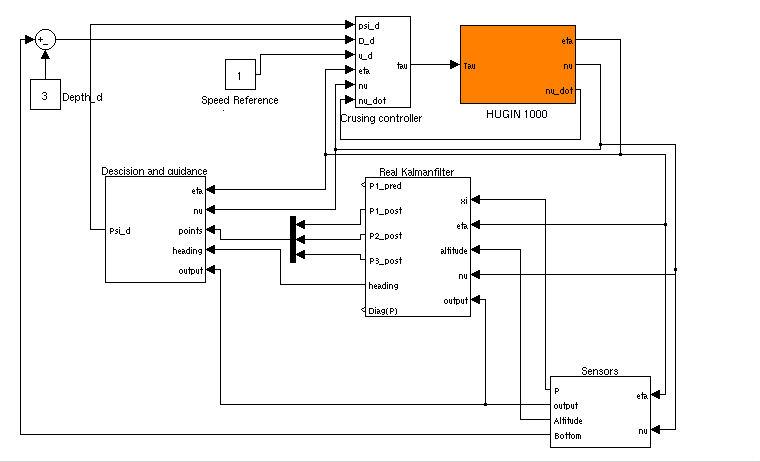
\includegraphics[width=\textwidth]{pics/simulink}
		\caption{The Simulink Diagram of the implemented Guidance System}
		\label{fig:ch3_simulink}
	\end{figure}
	The structure of the model are strictly modular and the blocks shown in the simulink diagram have the
	same function as in Figure~\ref{fig:ch2-blockdiagram}. This allows for updates and improved blocks
	to be implemented later, without designing a new system.
	
	The matlab-scripts are showen in the Appendix.
	

\section{Simulation Scenarios}
	To test the performance of the guidance system some scenarios are proposed. In all the scenarios, the
	pipeline are located at the sea bottom, around 10 meters bellow the surface. The depth is arbitrarily
	chosen and the value does change the scenarios except that the submerging time is longer. The AUV 
	will start at the surface and submerge towards the starting point of the mission. 
	\begin{description}
		\item[\textbf{1$^{\mathrm{st}}$ Scenario}.] The pipeline are at the exact location according 
		to predefined data. Environmental disturbances such as currents are turned off. The pipelien are
		continuously visible for the camera the whole inspection distance. Reference simulation.
		\item[\textbf{2$^{\mathrm{nd}}$ Scenario}.] Exact as over but with environmental forces turned on.
		\item[\textbf{3$^{\mathrm{rd}}$ Scenario}.] The pipeline are at the exact location where 
		it initially was laid. A section of the pipeline is buried and not visible for the camera.
		Environmental forces are turned on.
		\item[\textbf{4$^{\mathrm{th}}$ Scenario}.] The \'a priori information about the pipeline 
		are offset about 50 meteres to test the ability of the guidance system to search for the pipeline.
		Environmental forces are turned on.
	\end{description}


\section{Results}
	The matlab/simulink implementation were simulated with the given setup. A simulation were done to
	check if the low speed assumptions were valid. After this the simulation of the scenarios were done
	and produced the following results.


	\subsection{Test of the Low-speed Assumption}
		In figures \ref{fig:ch3_coriolis_forces} and \ref{fig:ch3_damping_forces} the forces and
		moments created by the Coriolis/centripetal and damping matrices are recorded. In Figure
		\ref{fig:ch3_coriolis_forces} the sway degree of freedom are dominant, and peaking about
		-400N during the turning manoeuvres of the AUV. The forces and moments created by the Coriolis
		terms are partially counteracted by the damping terms, that also have greater magnitude than
		the Coriolis terms.
		\begin{figure}[htbp]
			\centering
			\subfigure[Coriolis Forces]{
				\label{fig:ch3_coriolis_forces}
				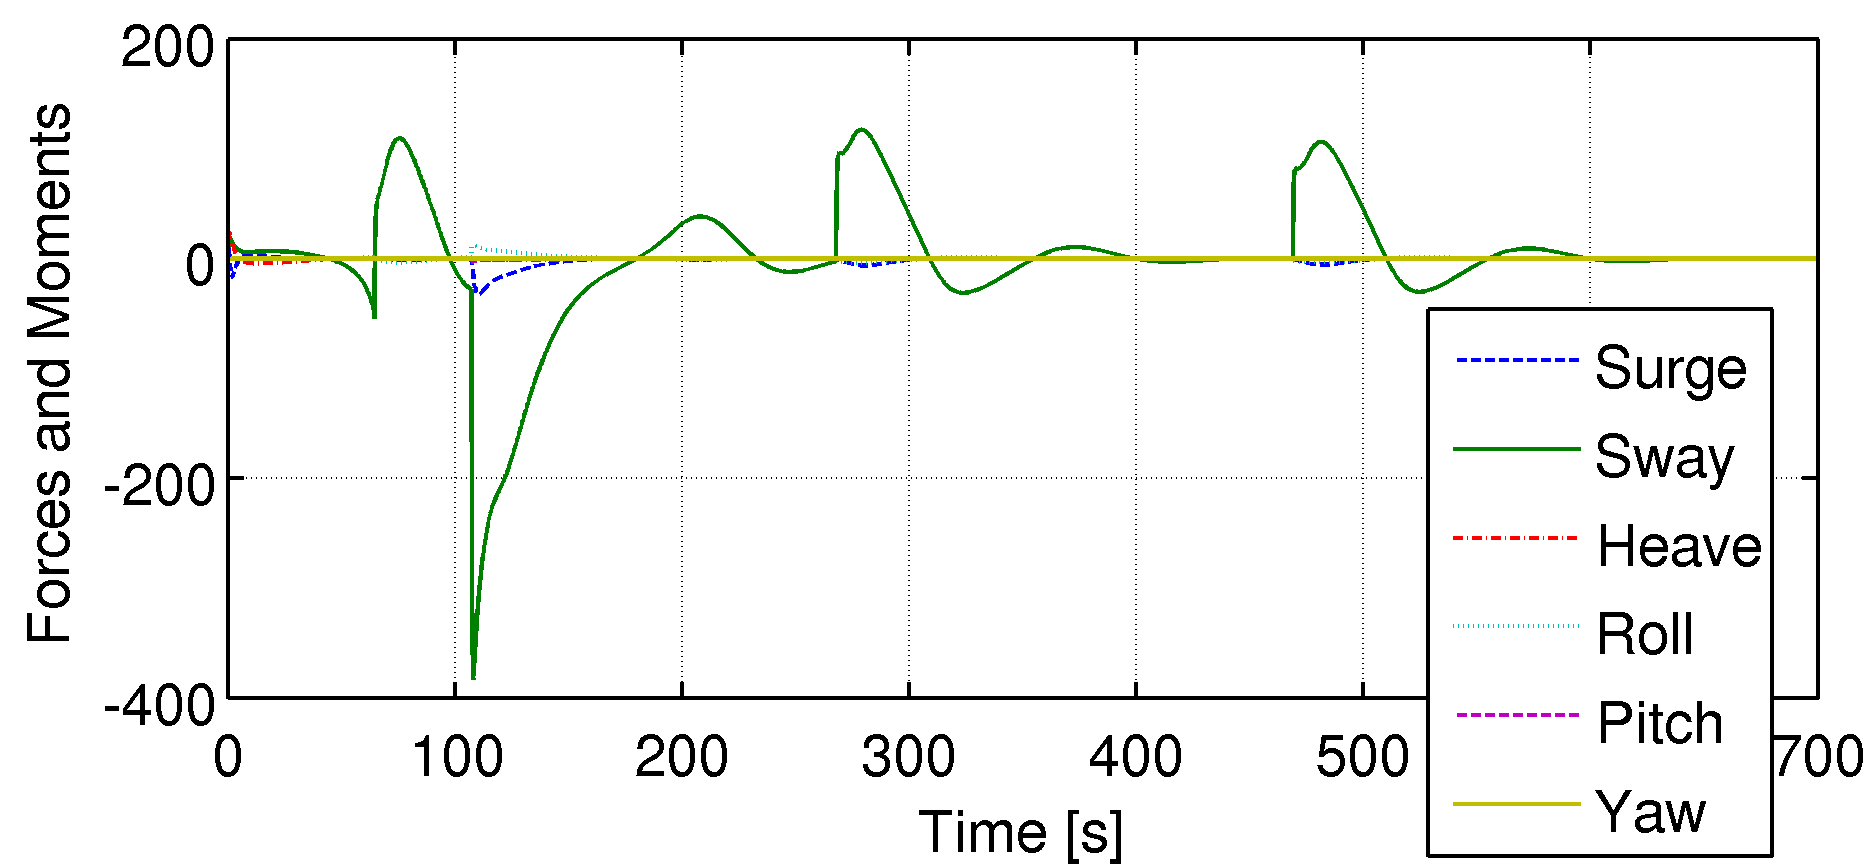
\includegraphics[width=0.7\textwidth]{pics/coriolis_forces}
			}	
			\subfigure[Damping Forces]{
				\label{fig:ch3_damping_forces}
				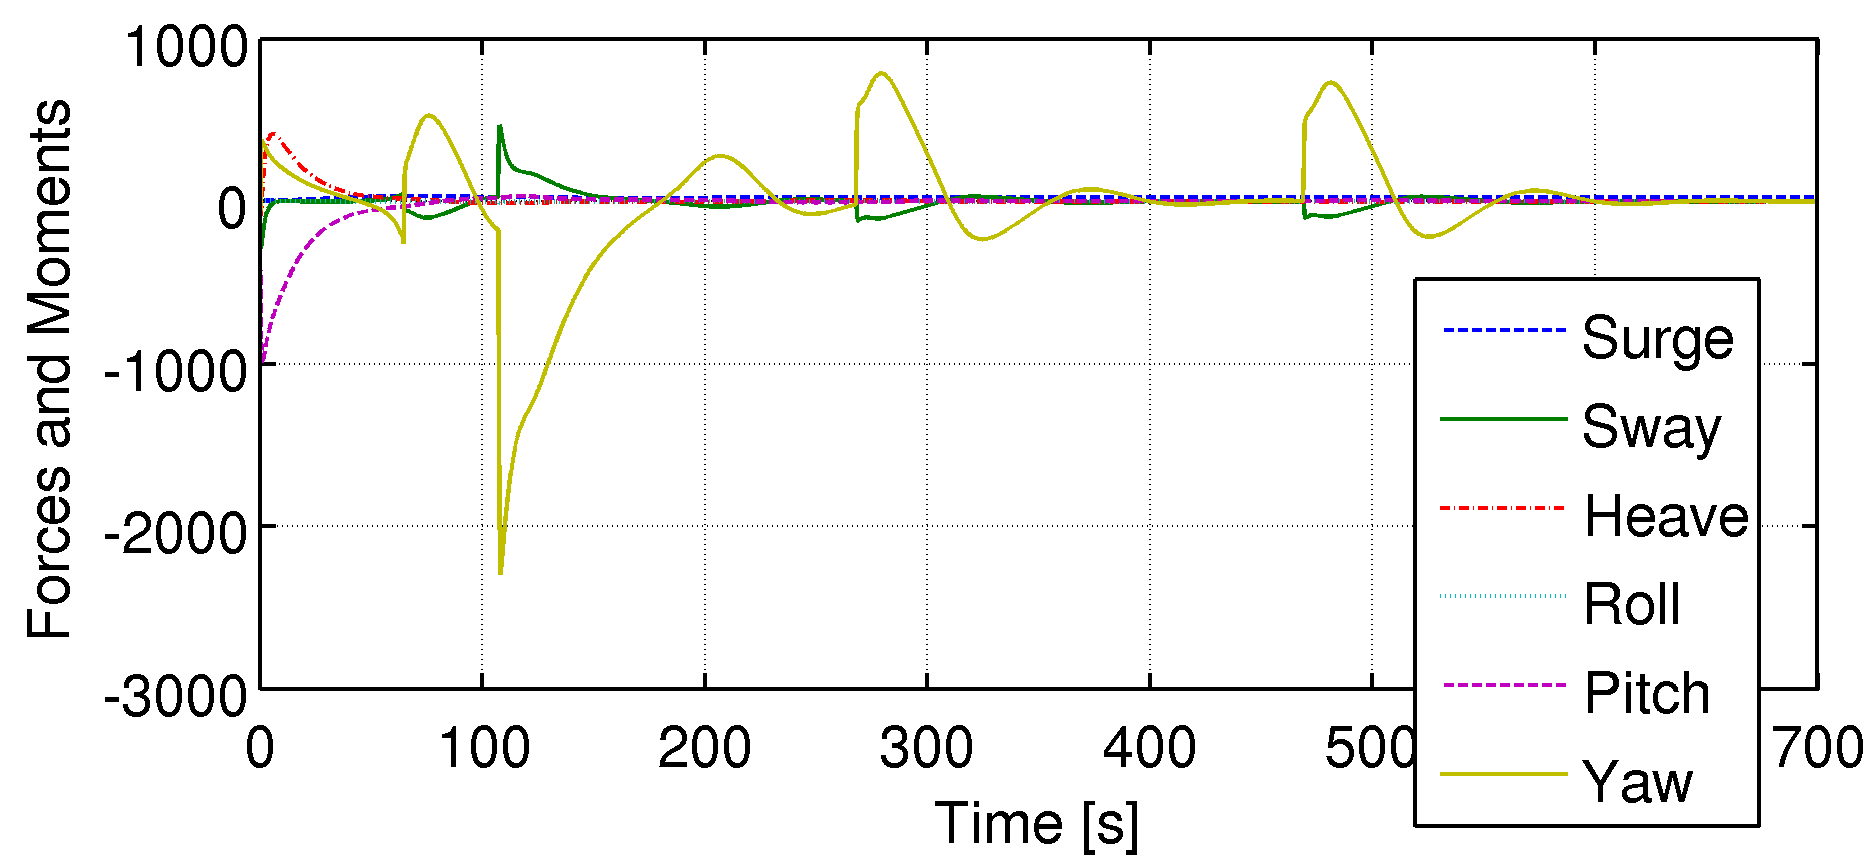
\includegraphics[width=0.7\textwidth]{pics/damping_forces}
			}
			\caption{The Forces associated with the AUV maneuvering}
			\label{fig:ch3-maneuvering forces}
		\end{figure}
		This suggests that the Coriolis/centripetal forces can be neglected and compensated for in the
		controller using integral terms.  

	\subsection{1$^{\mathrm{st}}$ Scenario}
		This is a reference test to see how the guidance system performs on the ideal case.
		This is to show the sensitivity to the environmental disturbances, introduced in later scenarios.
		\begin{figure}[htbp]
			\centering
			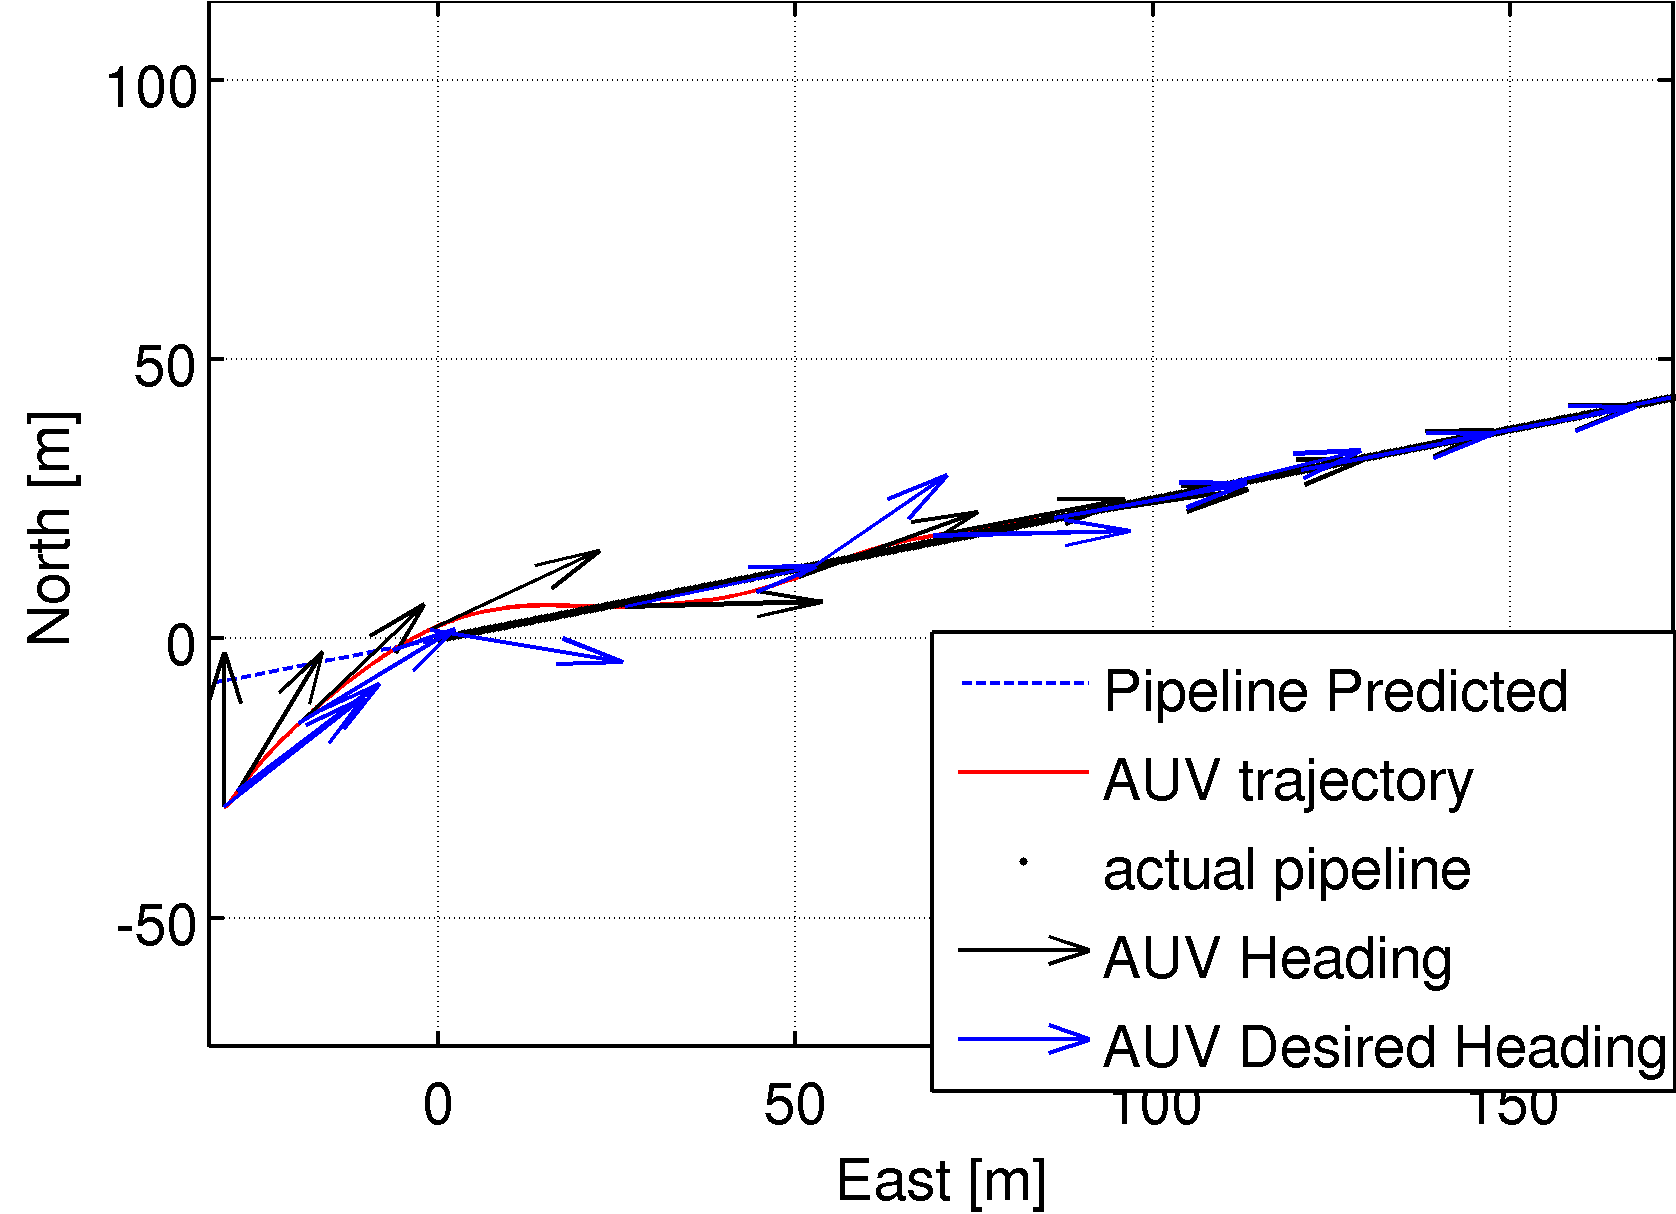
\includegraphics[width=0.7\textwidth]{pics/1st_NE_path}
			\caption{North East path of AUV without Current}
			\label{fig:ch3_1st_NE_path}
		\end{figure}
		\begin{figure}[htbp]
			\centering
			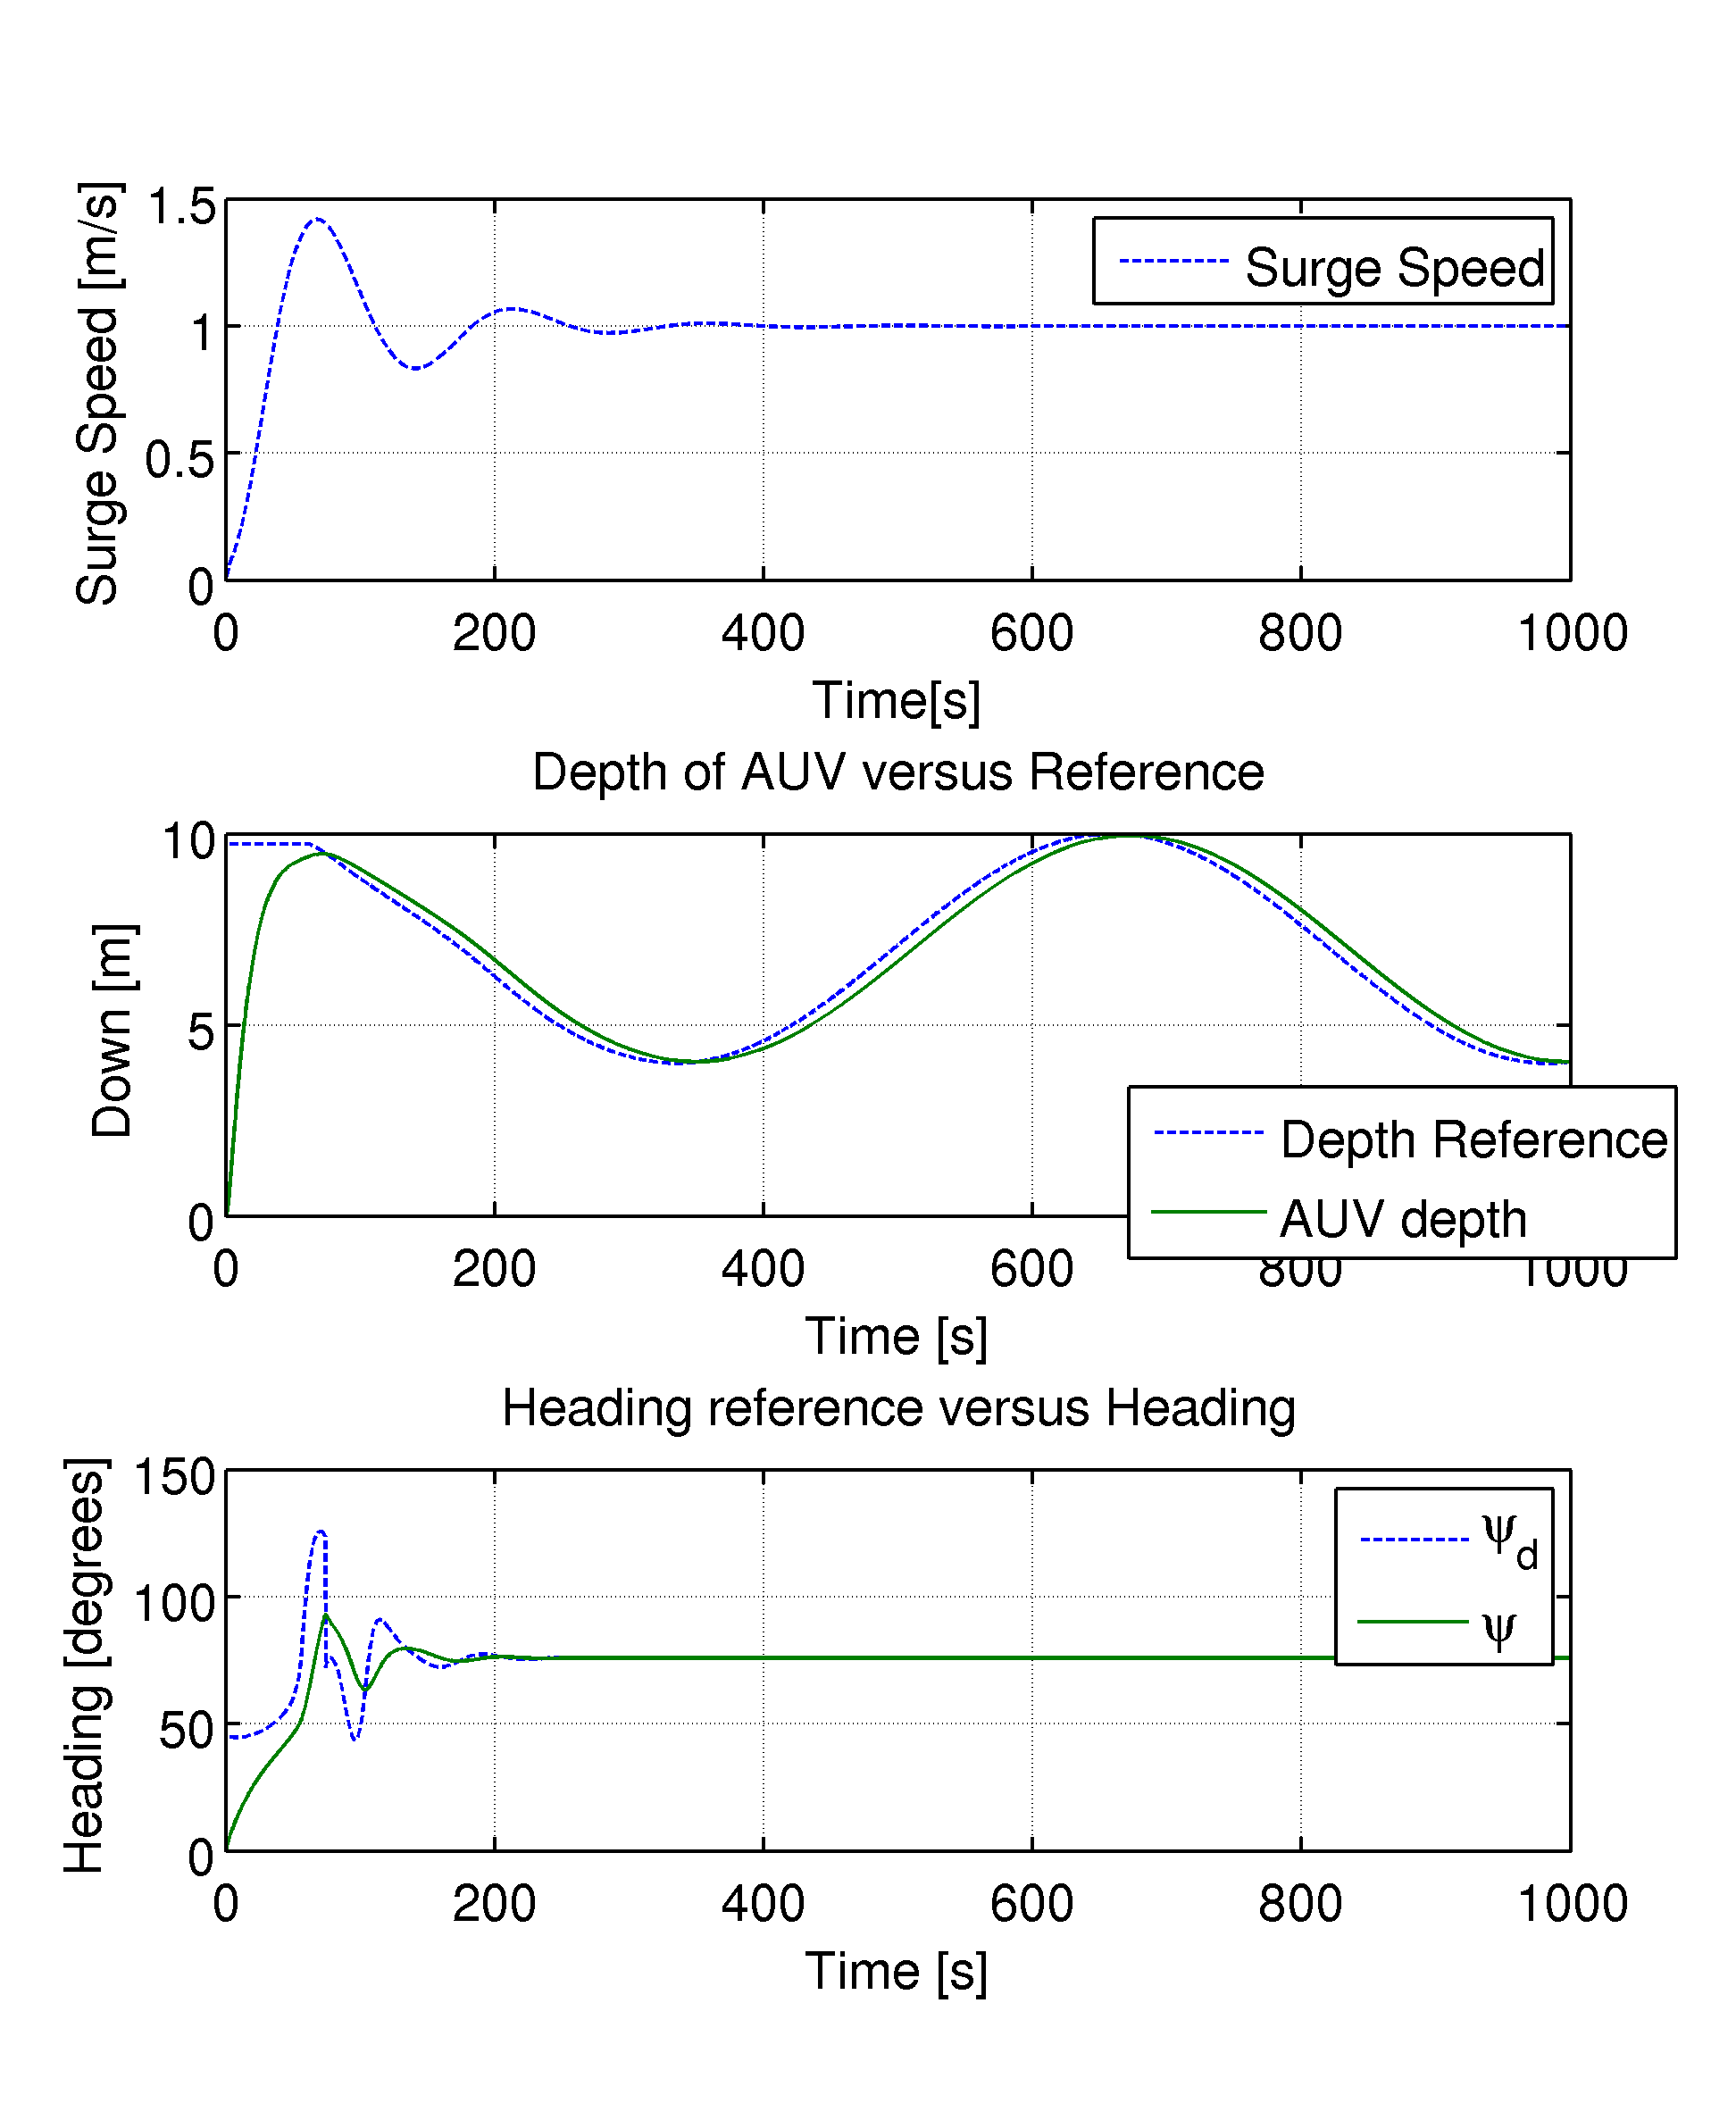
\includegraphics[width=0.75\textwidth]{pics/1st_uDpsi}
			\caption{Surge-, Depth- and Heading- Reference vs. Actual Values}
			\label{fig:ch3_1st_uDpsi}
		\end{figure}
		
		It can be seen from both Figure \ref{fig:ch3_1st_NE_path} and the
		third plot on Figure \ref{fig:ch3_1st_uDpsi} that the heading reference, $\psi_d$ have some
		oscillatory nature. This is because of the relatively low look-ahead distance defined in the
		guidance algorithm. This can be analogous to when driving a car and you fix your gaze on
		the road not very far ahead of the car, you will get more uneasy driving and jerking
		motion. 

		The depth reference is given by the bottom, created using a look-up table of a sinusoidal plane.
		The reference are followed pretty well. The delay on the
		action by the controller are created because the \textit{heave} direction are not directly
		controlled, but are relayed through the \textit{pitch} degree of freedom. This could probably
		have been reduced by feed-forwarding the reference into the controller as well. This will help
		the controller predict the motion and compensate for it when it happens.

		It is worth noting that the \textit{surge} speed overshoots, but is not seen as a problem for
		further simulation and analysis. The overshoot can be removed by including derivative action
		in the Speed controller. This would reduce the commanded force when reaching the set point.

	
	\subsection{2$^{\mathrm{nd}}$ Scenario}
		The environmental forces are now turned. The current is assumed only effective in the North
		East plane and has no effect in the \textit{heave}-direction. The current is moving from
		north-west to south-east, heading $-45^{\circ}$ and have a strength of $0.3$ m/s. 
		
		\begin{figure}[htbp]
			\subfigure[NE Path with	Waypoints]{\label{fig:ch3_2nd_NE_wpt}
				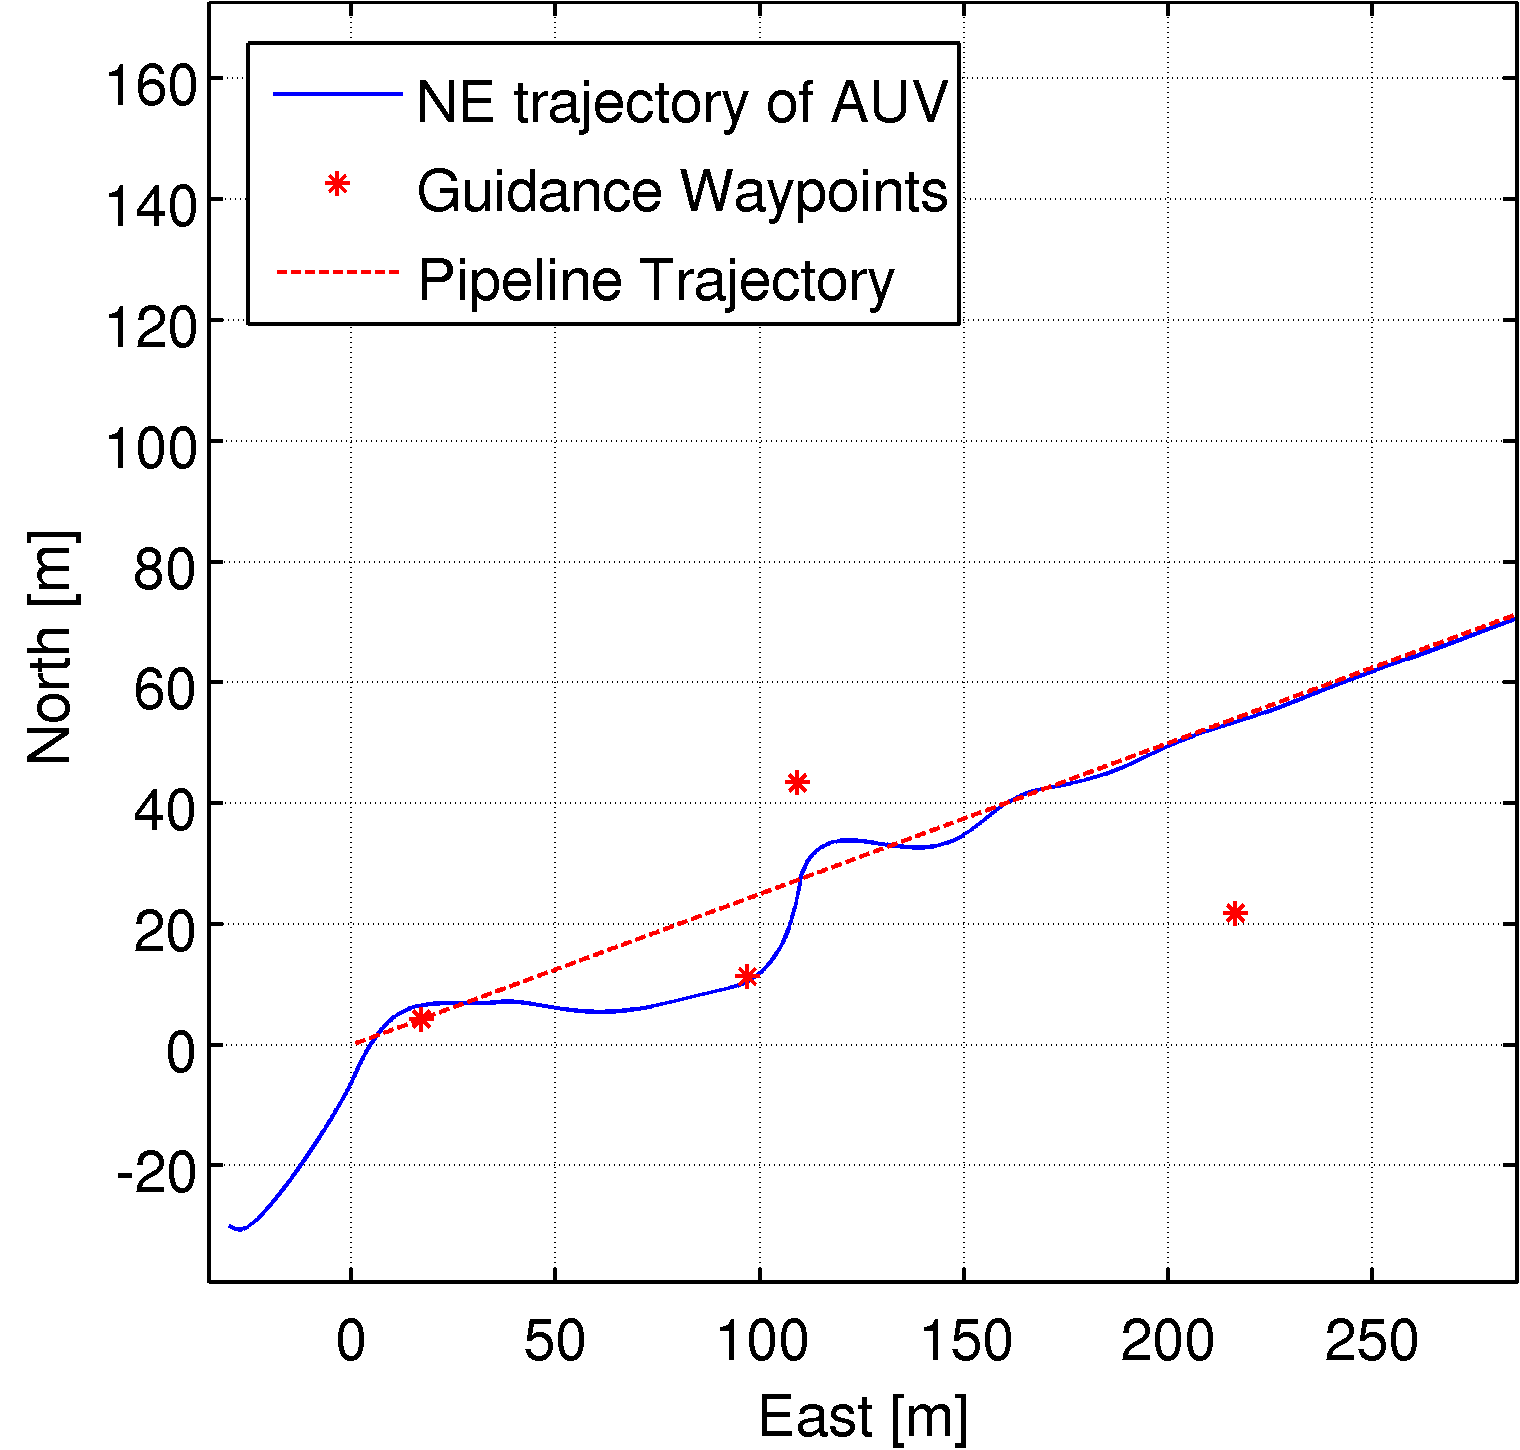
\includegraphics[width=0.5\textwidth]{pics/2nd_NE_wpt}}
			\subfigure[NE path with	Heading]{\label{fig:ch3_2nd_NE_path}
				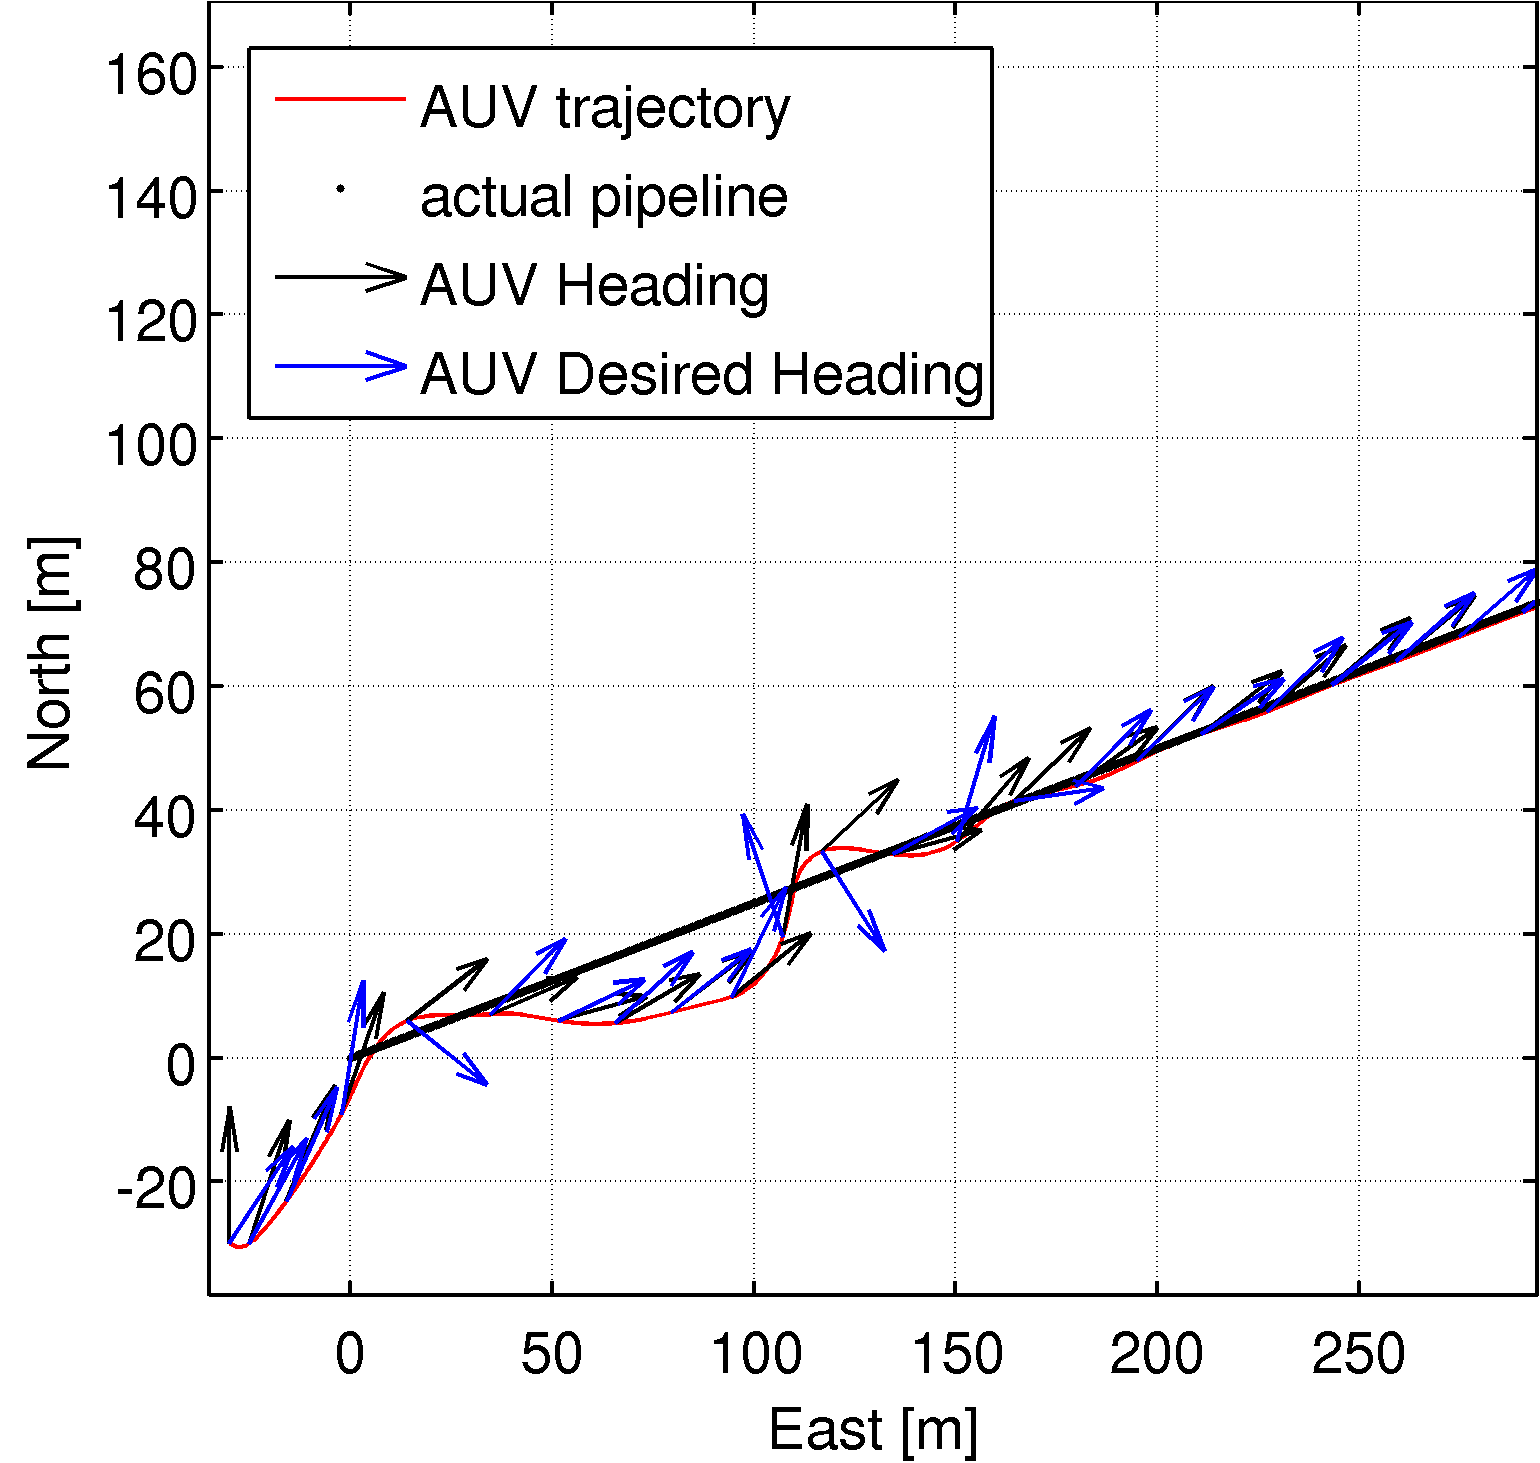
\includegraphics[width=0.5\textwidth]{pics/2nd_NE_path}} 
			\caption[Trajectory plots of the 2nd scenario]{Plots of the AUV Showing Trajectory, 
			Guidance Waypoints and Heading of AUV second scenario}
			\label{fig:ch3_2nd_NE_plots}
		\end{figure}
		In Figure \ref{fig:ch3_2nd_NE_wpt} the search waypoints are shown. The reason for the extra
		``de-tour'' away from the pipeline are because of the short time delay before considering the
		pipeline lost. As seen in the first Scenario there are oscillations in the heading reference.
		This causes the AUV to drift off the pipeline trajectory and therefor lose visual contact
		with it. The system considers the pipeline as lost and generates a search pattern, the
		``divergent zig-zag'' spoken of in Chapter \ref{subsec:ch2_searchpattern}. The time before
		going into search mode are set to 25 seconds.

		\begin{figure}[htbp]
			\centering
			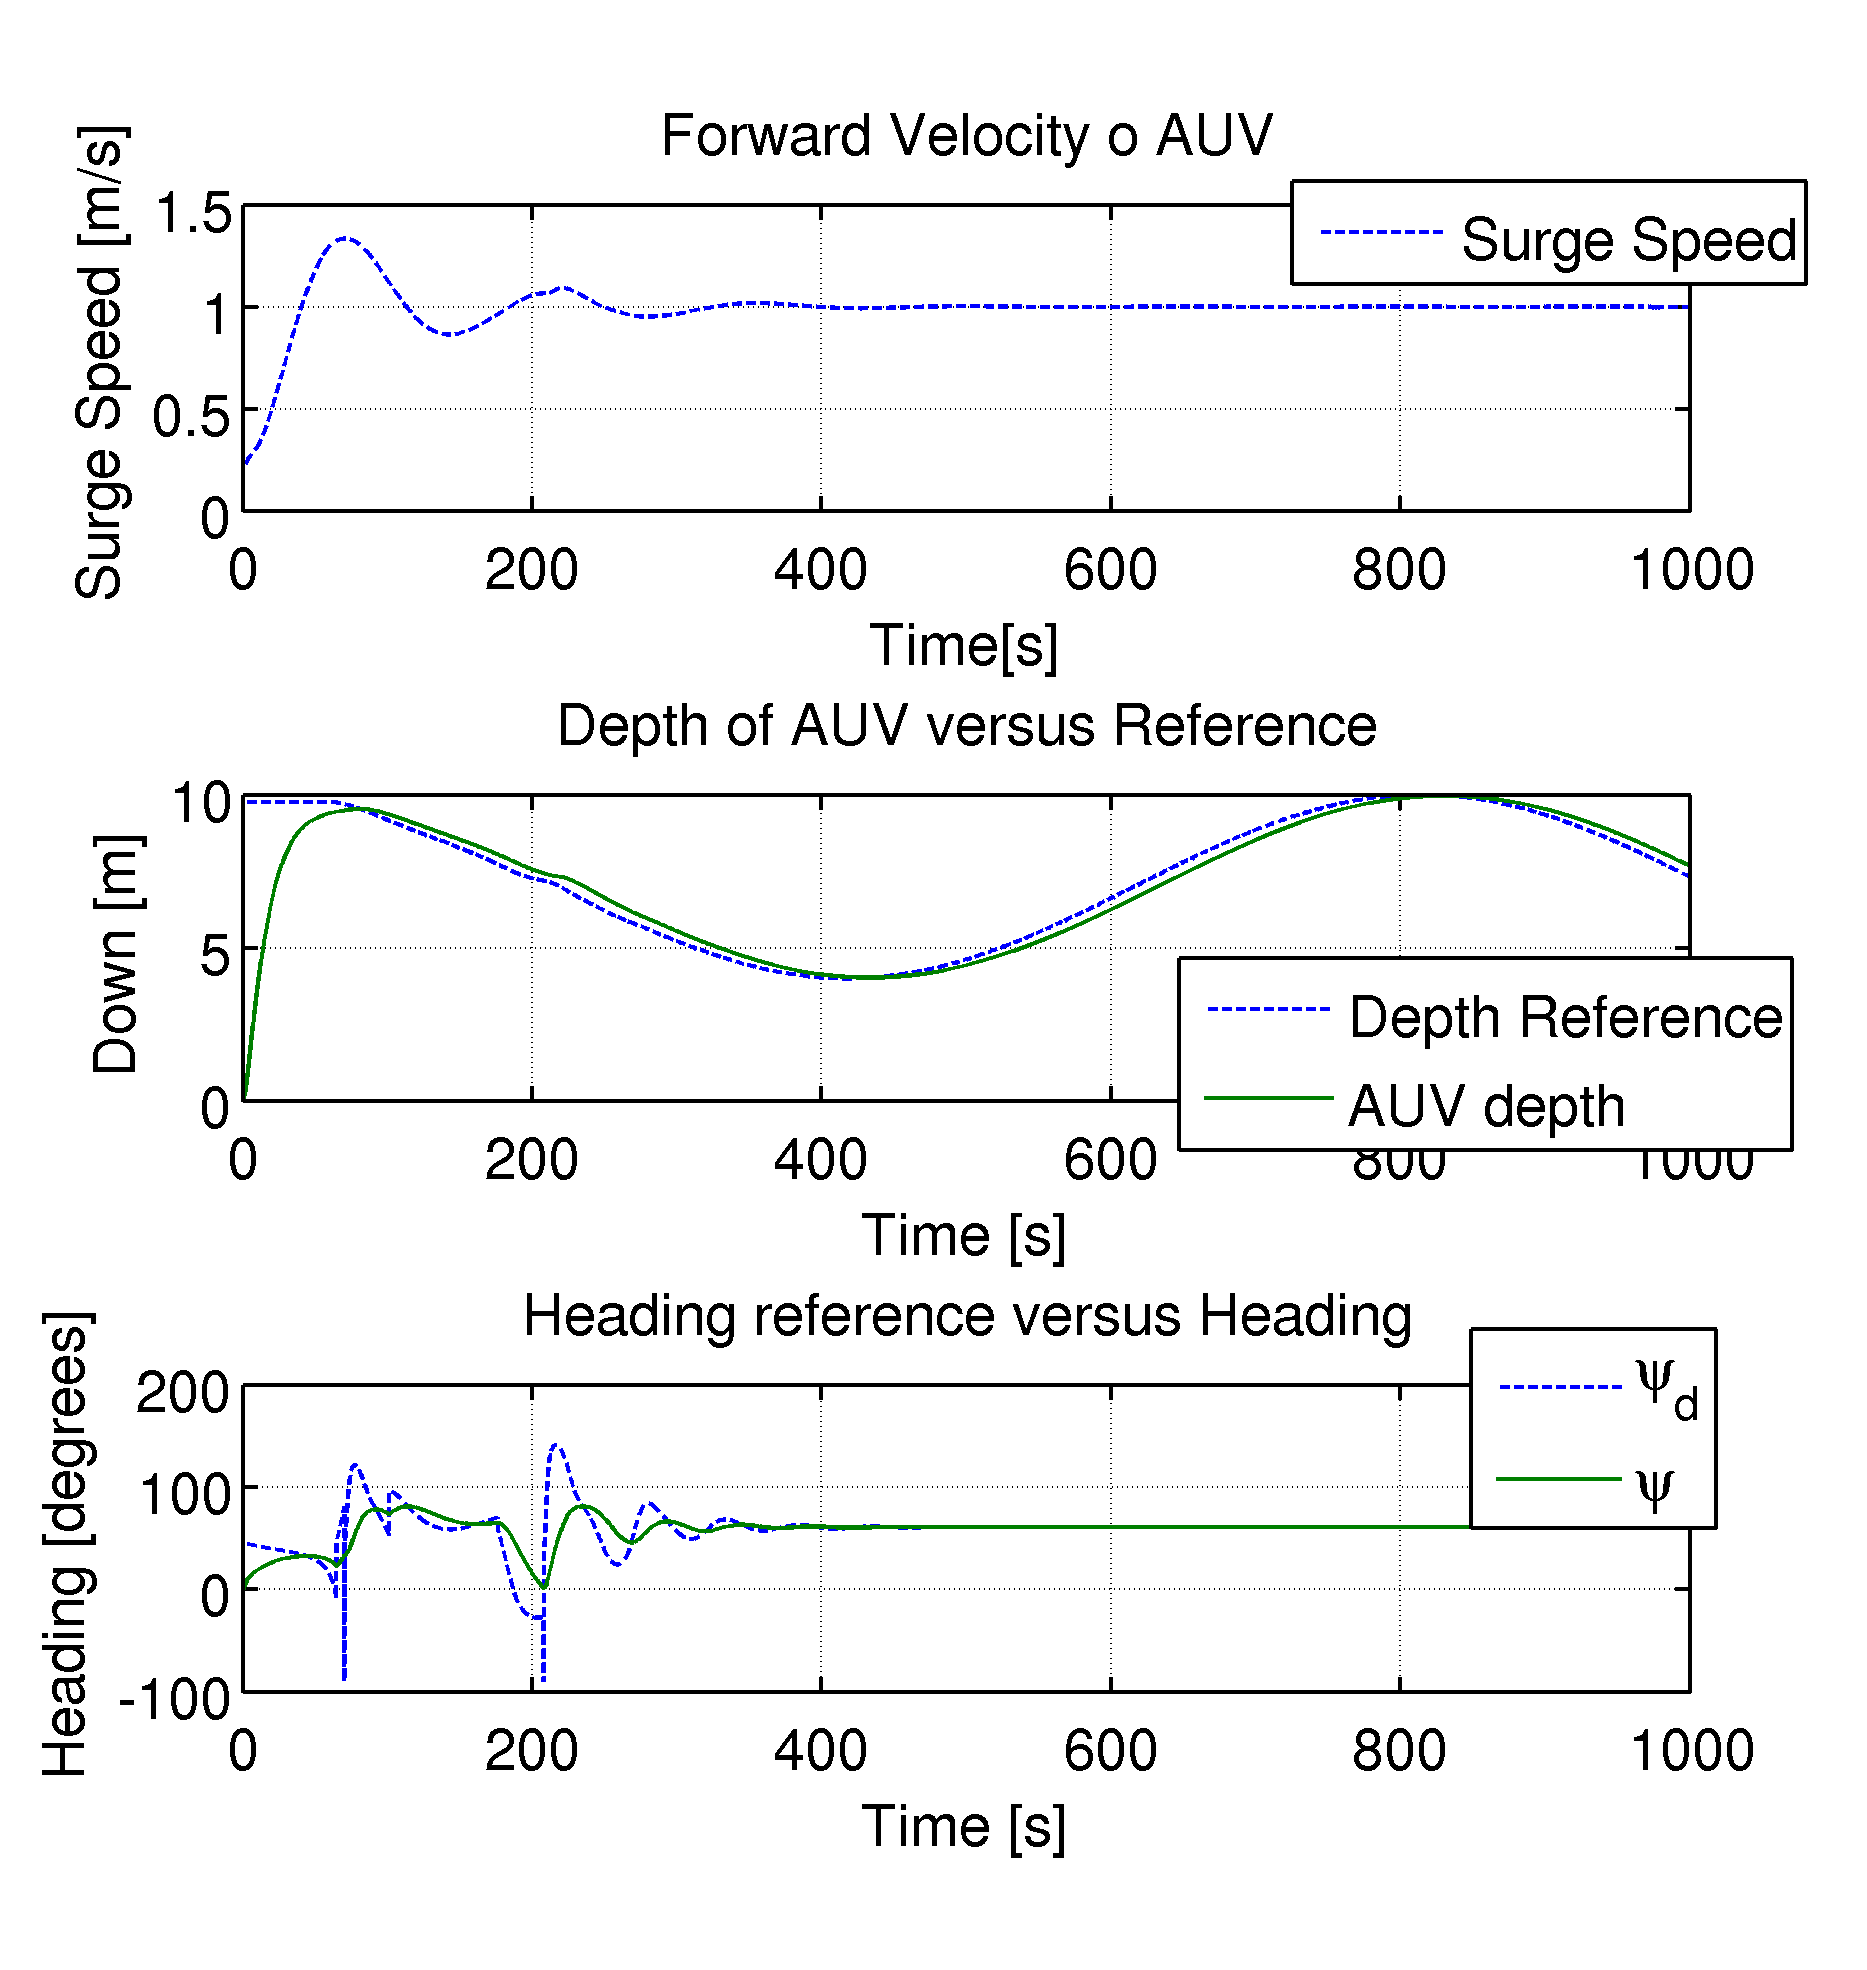
\includegraphics[width=0.70\textwidth]{pics/2nd_uDpsi}
			\caption[Reference plots for the 2nd scenario]{Surge-, Depth- and Heading- 
			Reference with Current influence second scenario}
			\label{fig:ch3_2nd_uDpsi}
		\end{figure}
		When current are introduced the AUV heading are ``leaned'' toward the current. In
		Figure~\ref{fig:ch3_2nd_NE_path} the current are coming from north-west, corresponding to
		the upper right corner in the figure. This current will try to push the
		AUV off the pipeline. The guidance system answers this disturbance by adjusting the heading
		reference towards the current. This is one of the reasons why the lookahead distance are
		chosen small, because of this the AUV will not drift far away from the pipeline. Since the
		current is constant, a equilibrium is achieved between the desired heading and the
		current. The heading converges towards around $60^{\circ}$ instead of the pipeline direction
		of $75^{\circ}$.

		The AUV are not directly on top of the pipeline anymore, but it is not desirable to be exactly
		over the pipeline all the time. To strictly control the AUV to lay exactly over the pipeline
		would use much of the limited power supply. Also, the objective of the AUV are not to stay
		exactly over the pipeline, but to provide good pictures and sensor data for later inspection 
		by humans. It might be much easier to analyse a stable picture than a tightly regulated
		motion which might cause a noisy picture. 

		%\begin{figure}[htbp]
		%	\centering
		%	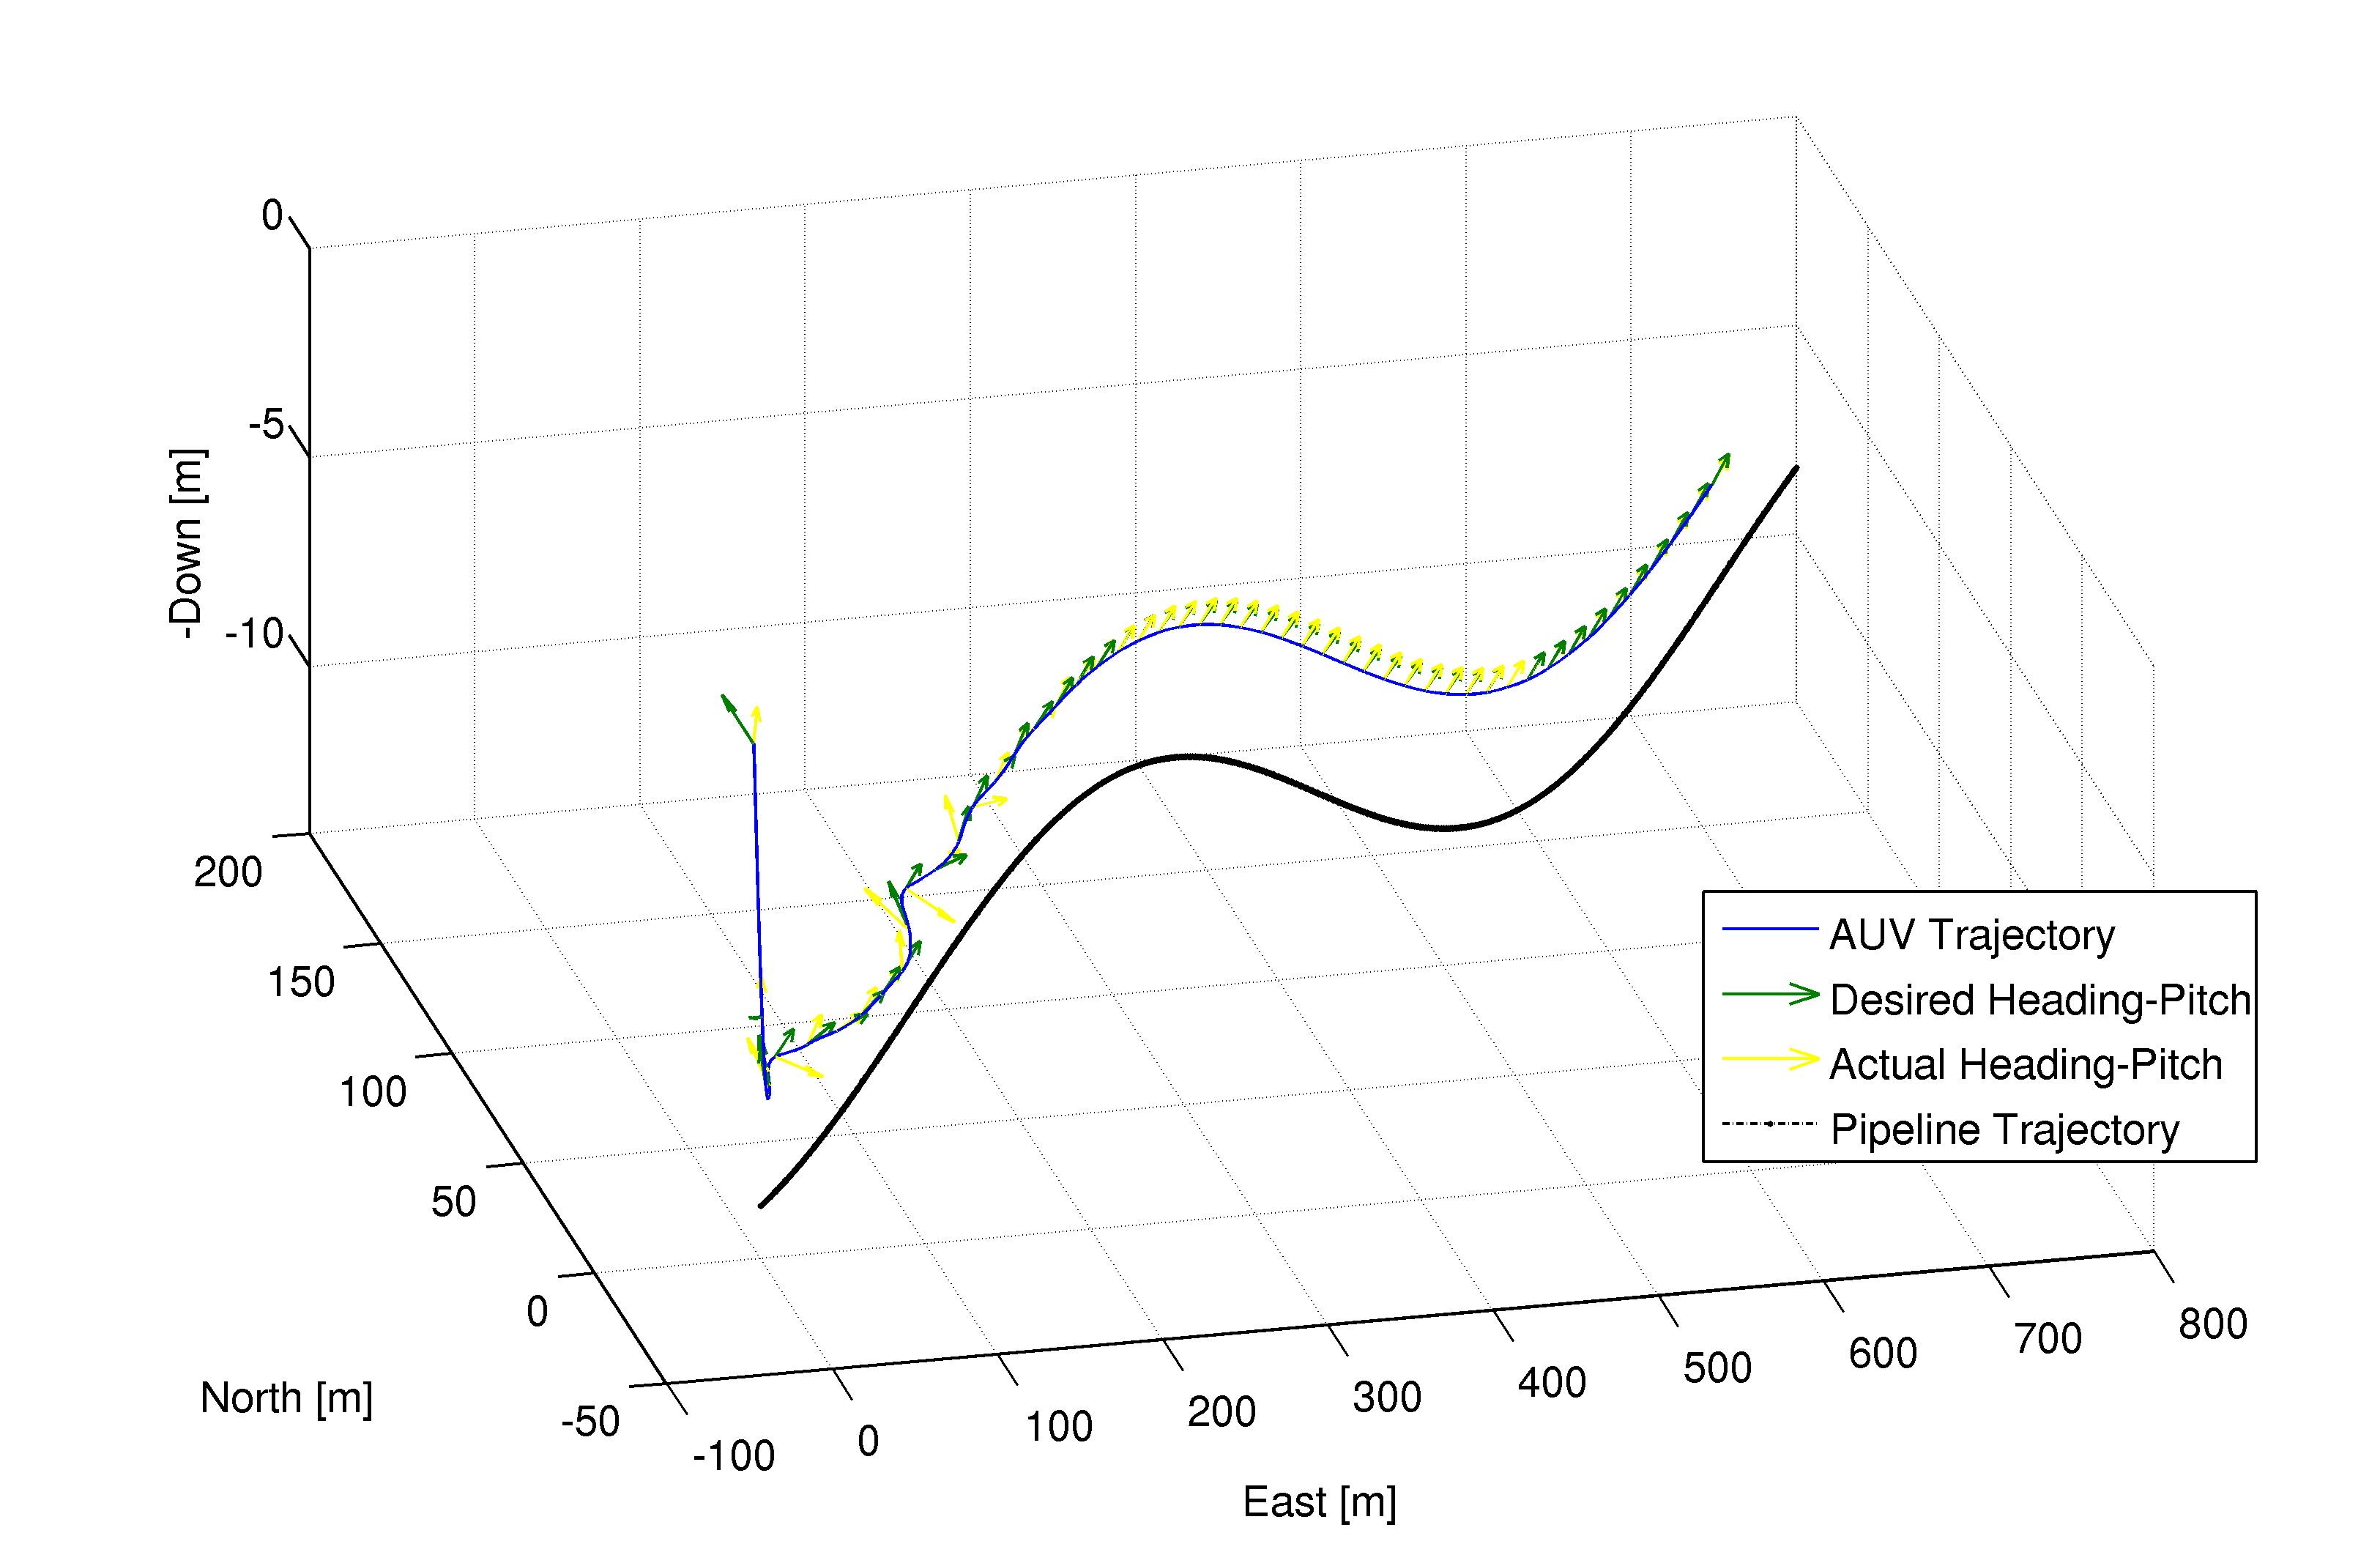
\includegraphics[width=0.95\textwidth]{pics/2nd_3d_plot}
		%	\caption{3D plot of the AUV Movement}
		%	\label{fig:ch3_2nd_3d_plot}
		%\end{figure}
		%In Figure \ref{fig:ch3_2nd_3d_plot} the 3D trajectory of the AUV are shown, togheter with the
		%actual pipeline trajectory. 
	

	\subsection{3$^{\mathrm{rd}}$ Scenario}
		The setup for this scenario, is a simulated burrial of the pipeline at approximately $50$
		meters North and $200$ meters East. At this point the camera looses track of the pipeline. The
		guidance system will command the AUV to continue following the predicted pipeline until some
		time limit are reached. This time limit are set to $60$ seconds. From Figure
		\ref{fig:ch3_3rd_NE_plots} it can be seen that the AUV follows the predicted pipeline for
		about $50$ meters and then engages in the predetermined search pattern.
		\begin{figure}[htbp]
			\centering
			\subfigure[NE Path with	Waypoints]{\label{fig:ch3_3rd_NE_wpt}
				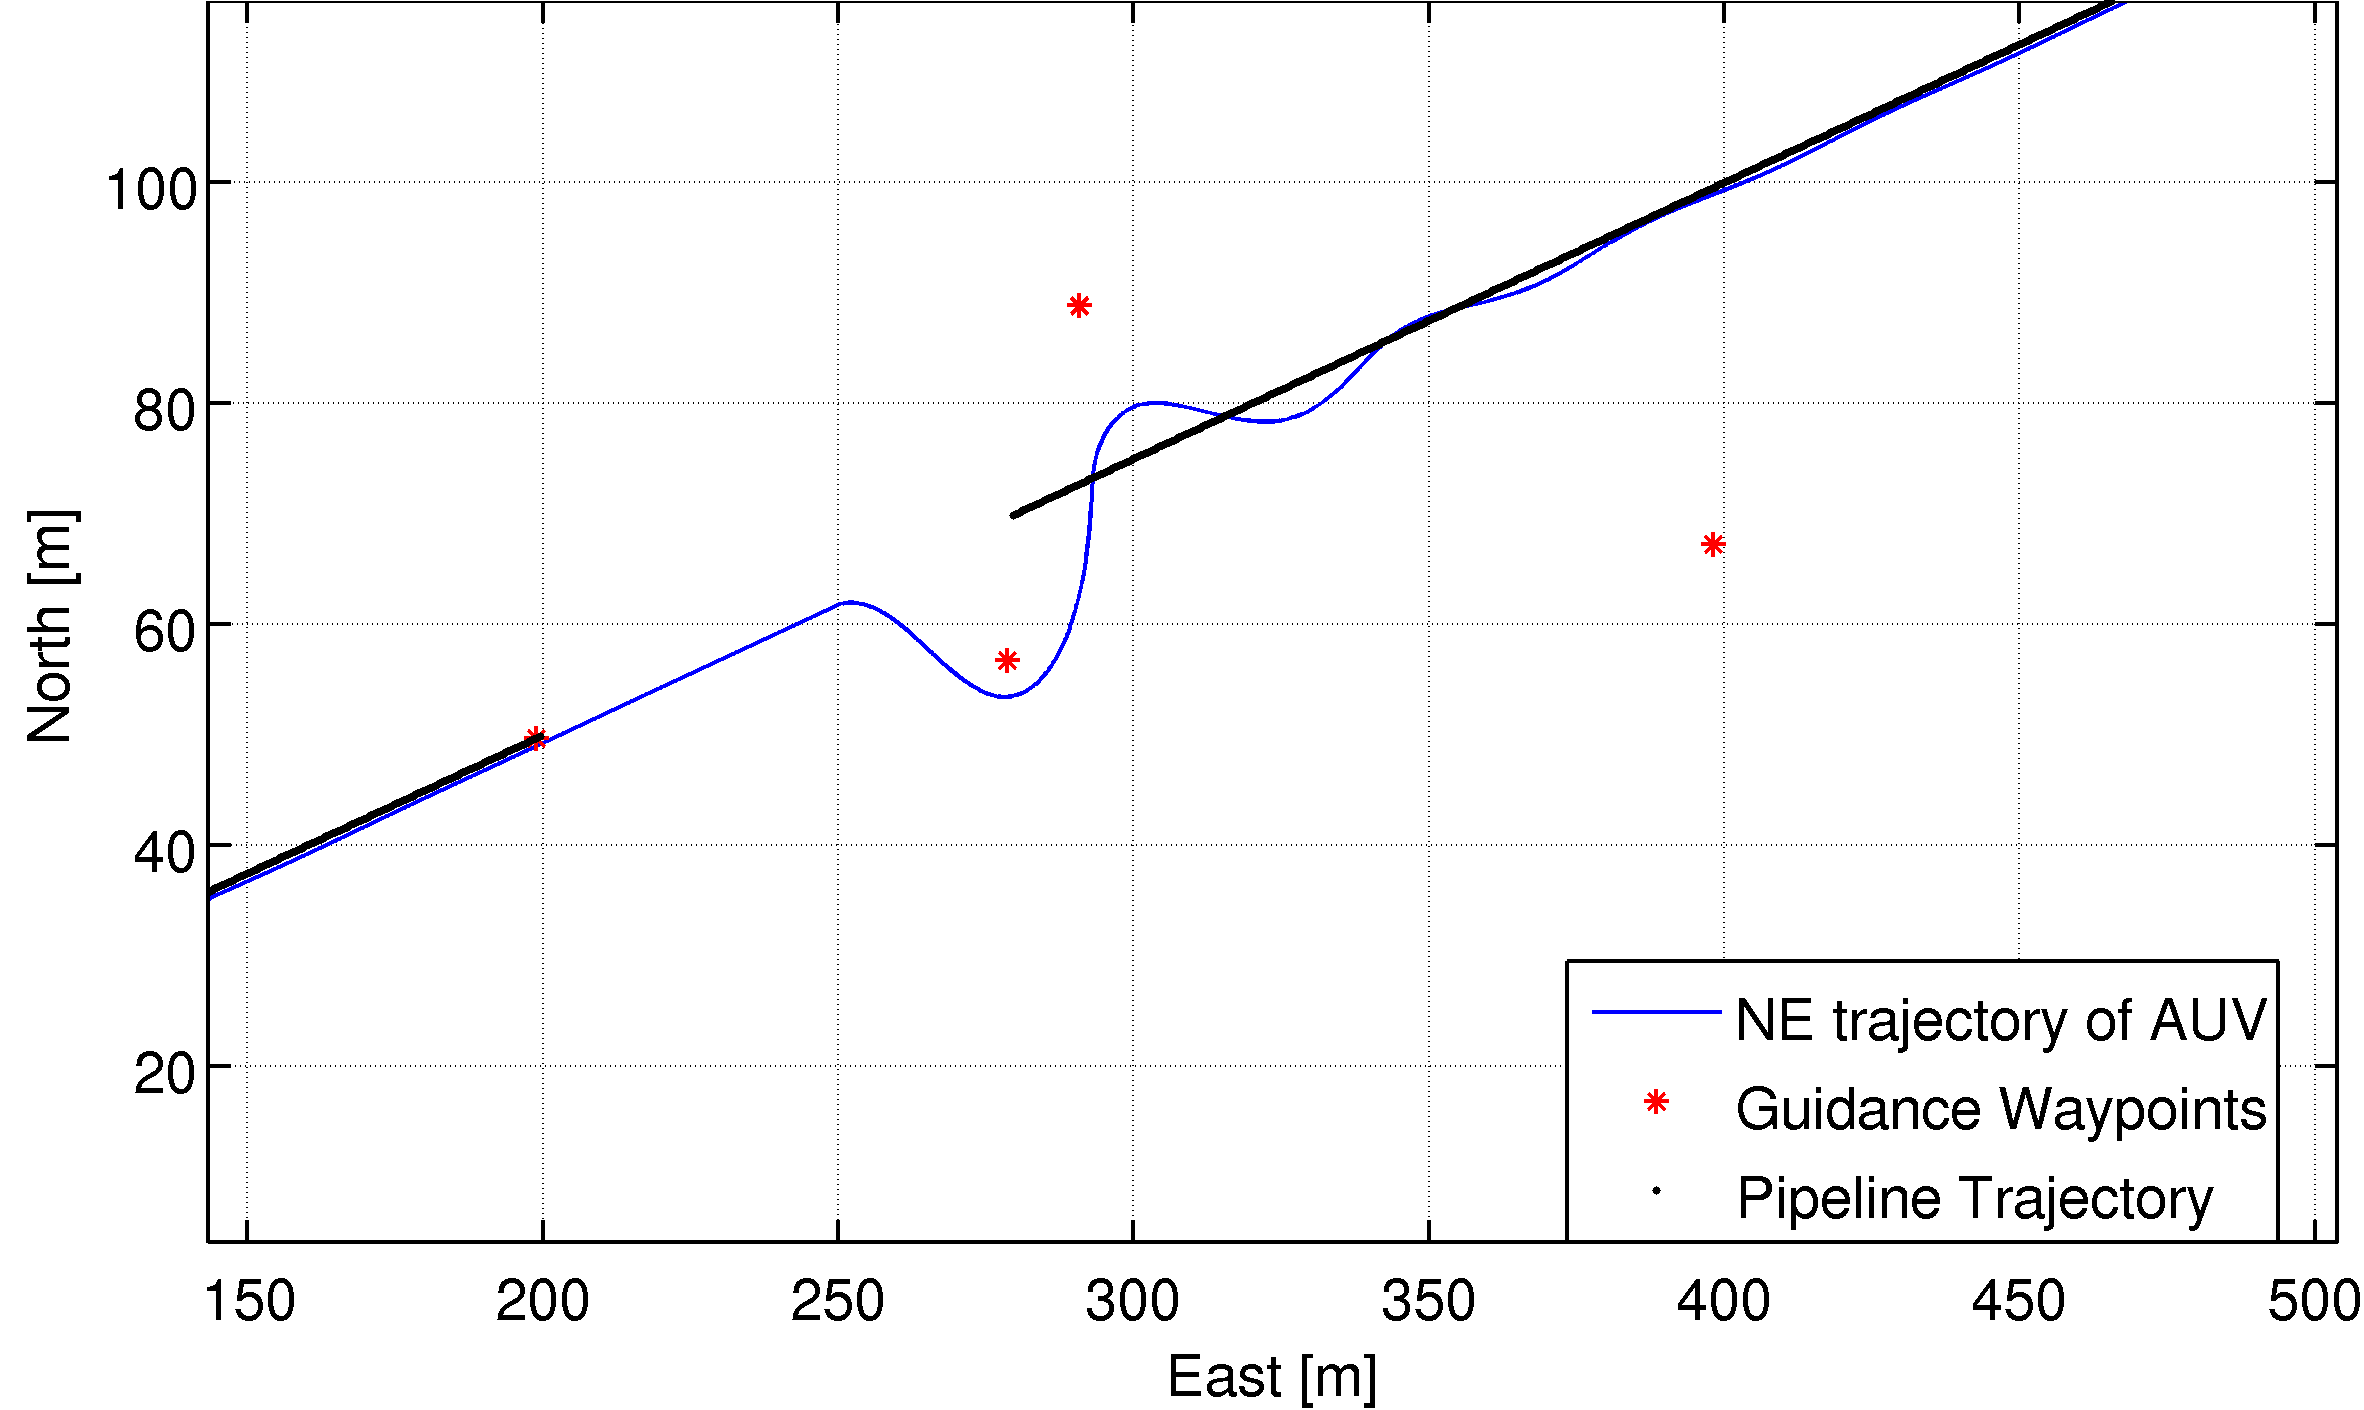
\includegraphics[width=0.7\textwidth]{pics/3rd_NE_wpt}}
			\subfigure[NE path with	Heading]{\label{fig:ch3_3rd_NE_path}
				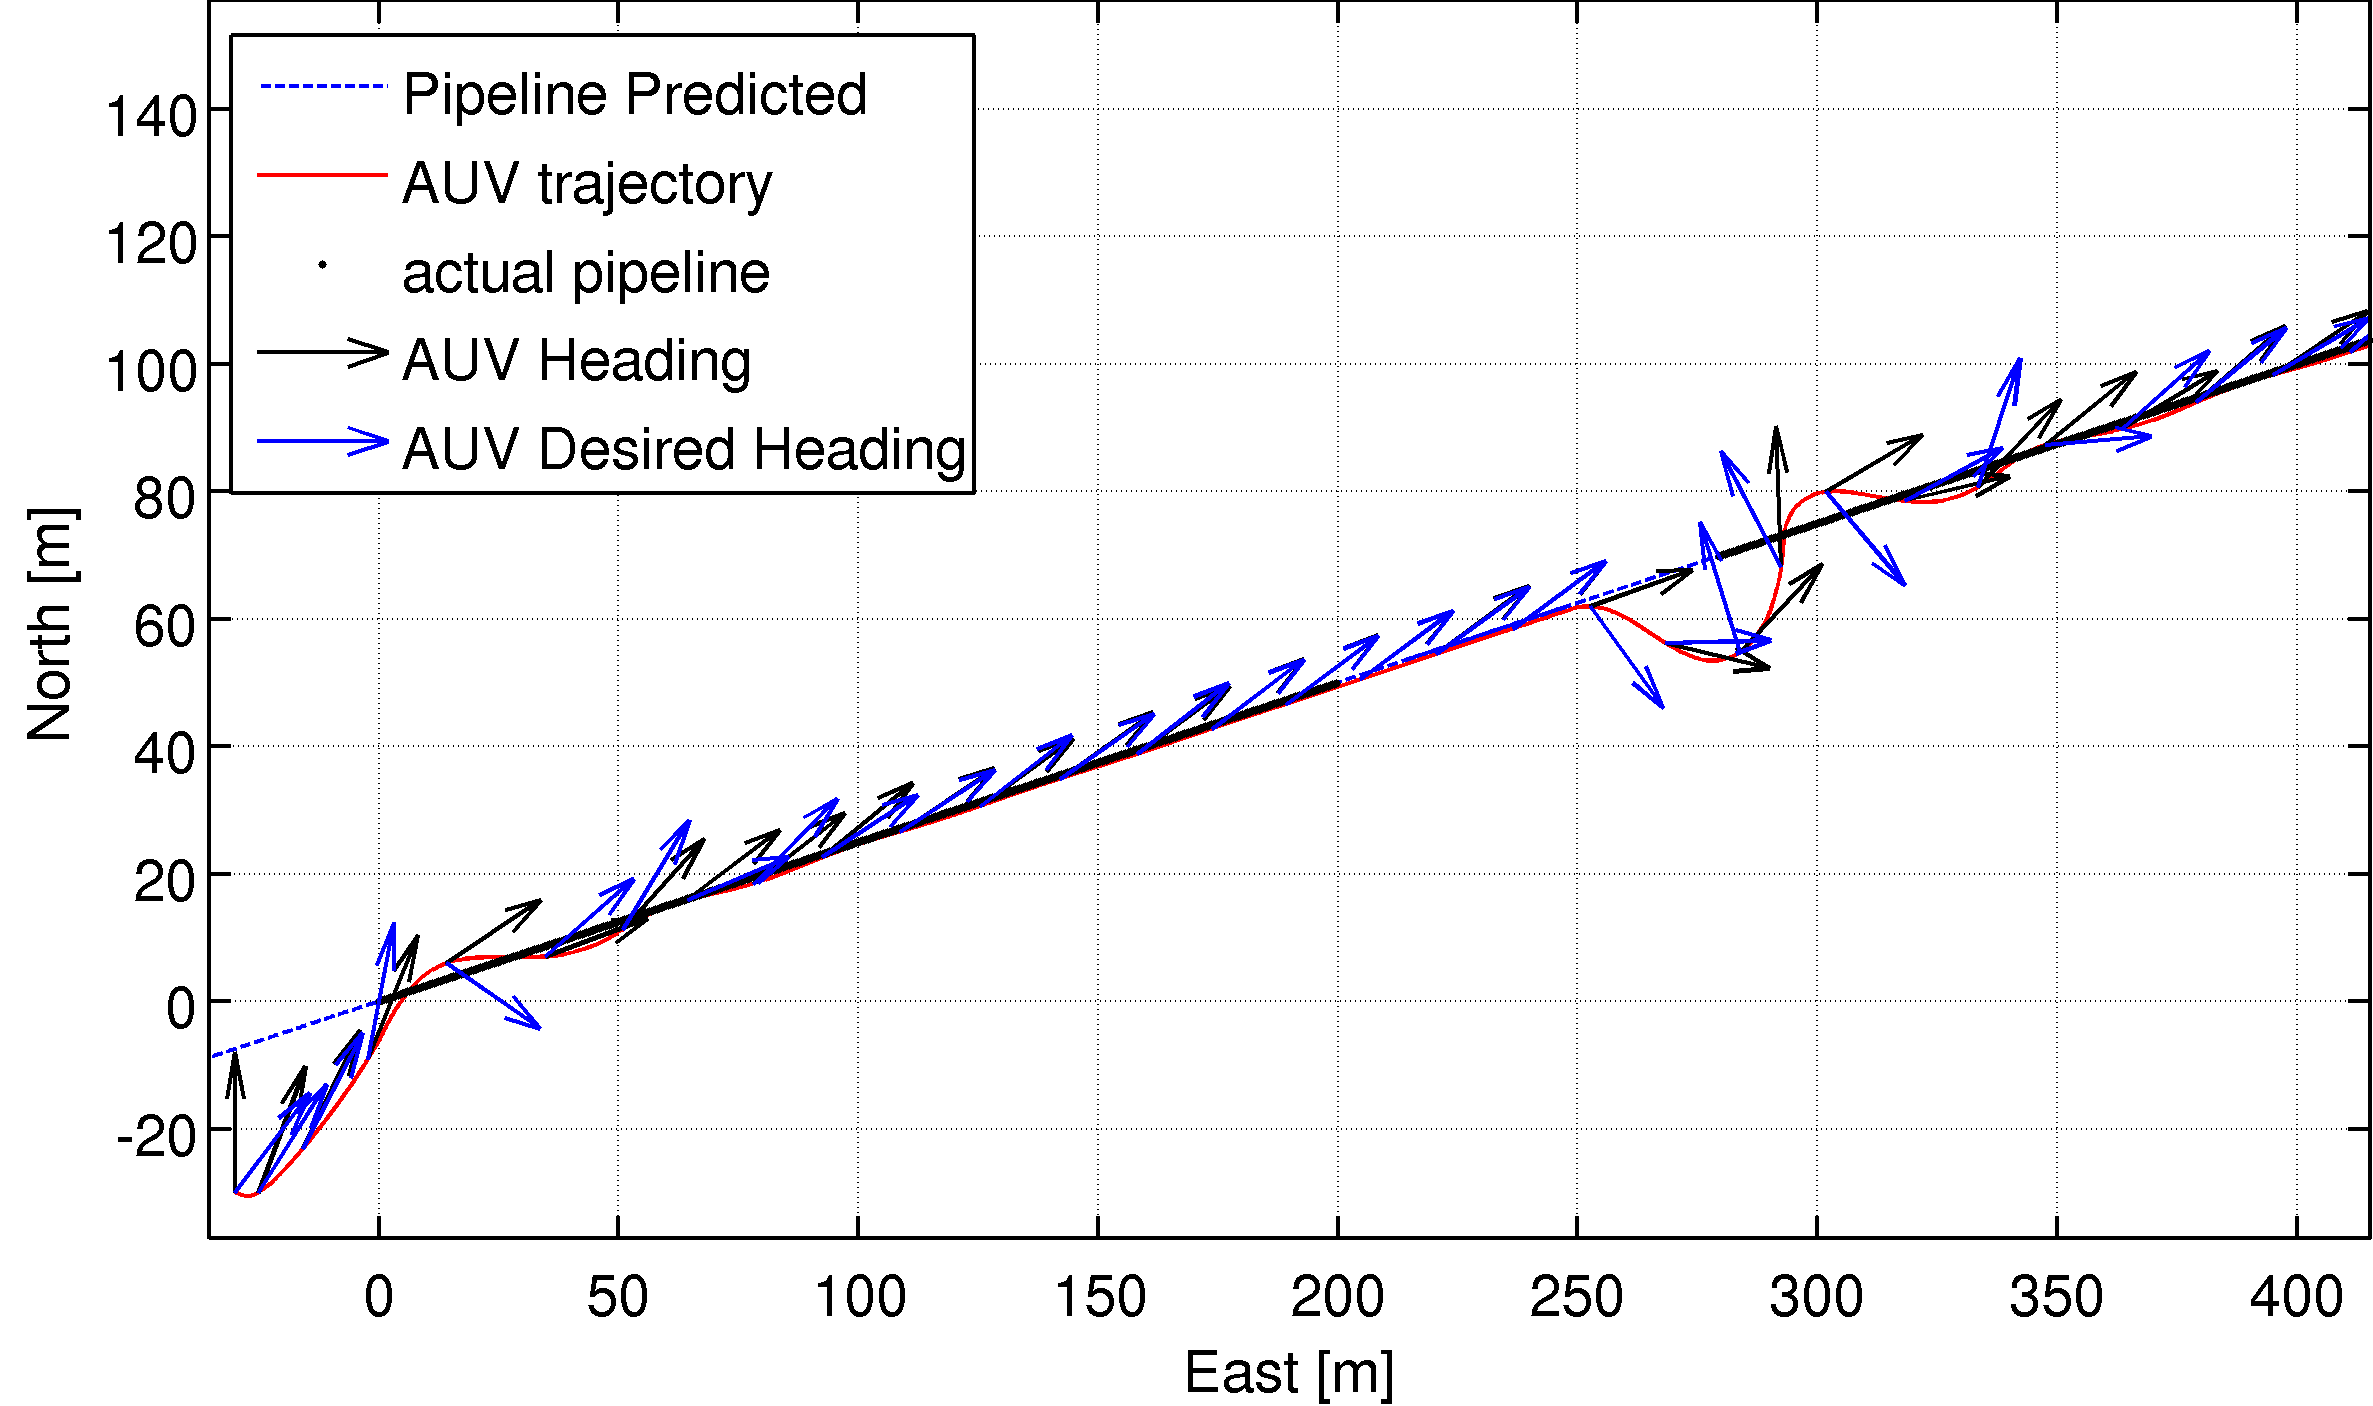
\includegraphics[width=0.7\textwidth]{pics/3rd_NE_path}} 
			\caption[Trajectory plots from the 3rd scenario]{Plots of the AUV Showing Trajectory, 
			Guidance Waypoints and Heading of AUV for the 3$^{\mathrm{rd}}$ Scenario}
			\label{fig:ch3_3rd_NE_plots}
		\end{figure}
		
		The meaning of following the predicted pipeline is of course to get back on track at the end
of
		the buried stretch. Sometimes pipelines are buried on purpose to seal them from environmental
		erosion, and sometimes this happens unintended. In
		either case, the need of more sensors which can penetrate the sea bottom and locate the
		pipeline are needed. 

		There are no turning trajectory implemented at this point, and will not be used in
		the next scenarios either.
		
	
	
	\subsection{4$^{\mathrm{th}}$ Scenario}
		The fourth Scenario is to demonstrate the capabilities for the AUV to acquire the pipeline,
		when the pipeline is offset from where it was thought to be. 
		
		\begin{figure}[htbp]
			\centering
			\subfigure[NE Path with	Waypoints]{\label{fig:ch3_4th_NE_wpt}	
				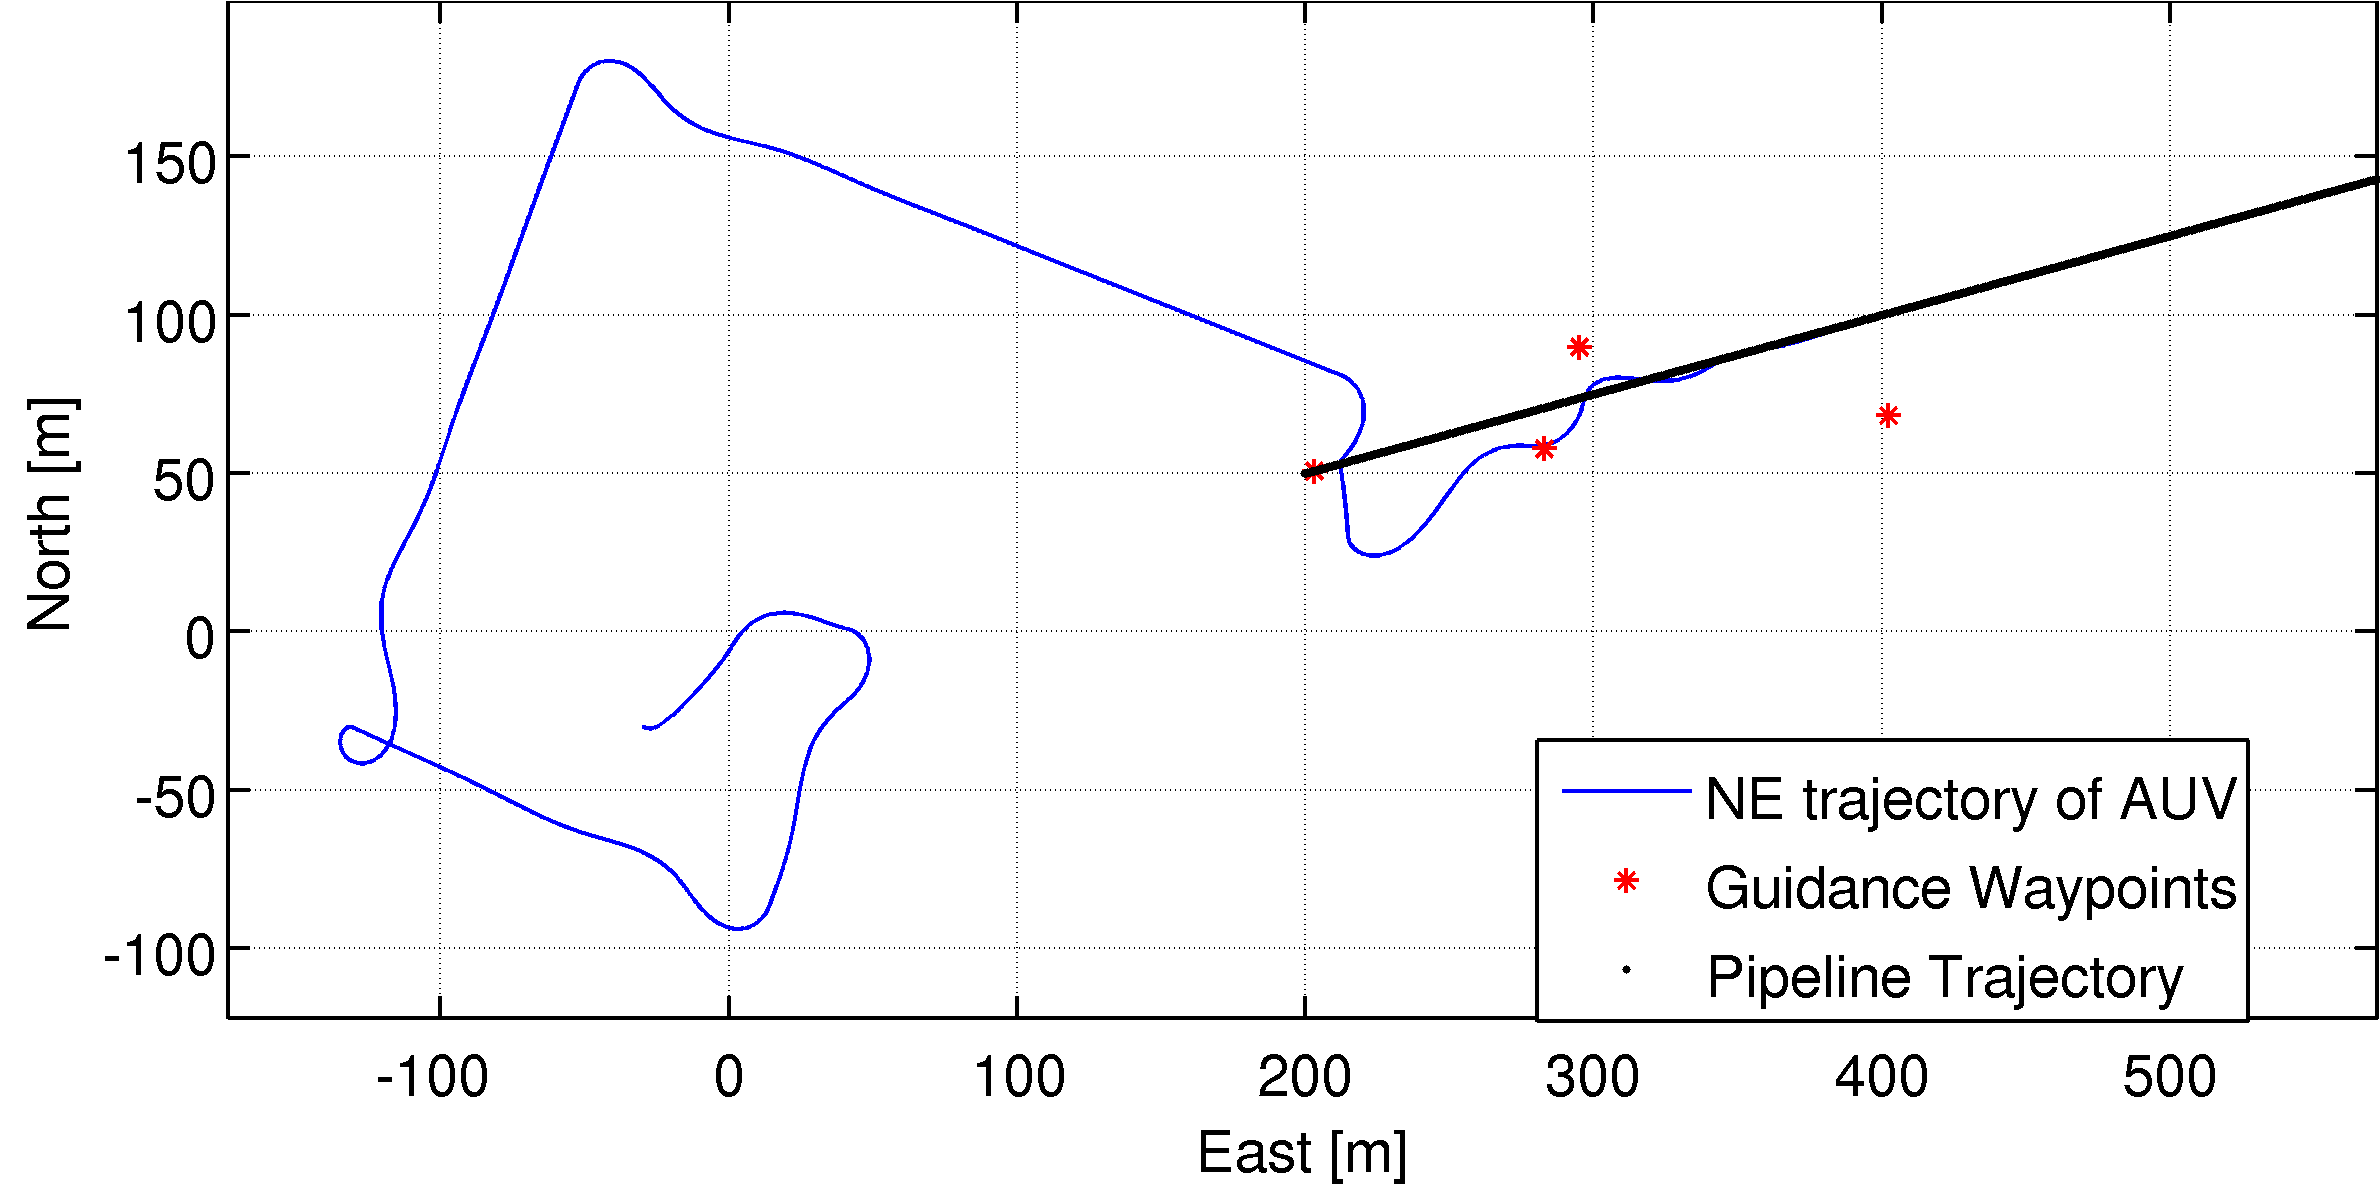
\includegraphics[width=0.8\textwidth]{pics/4th_NE_wpt}}
			\subfigure[NE path with	Heading]{\label{fig:ch3_4th_NE_path}
				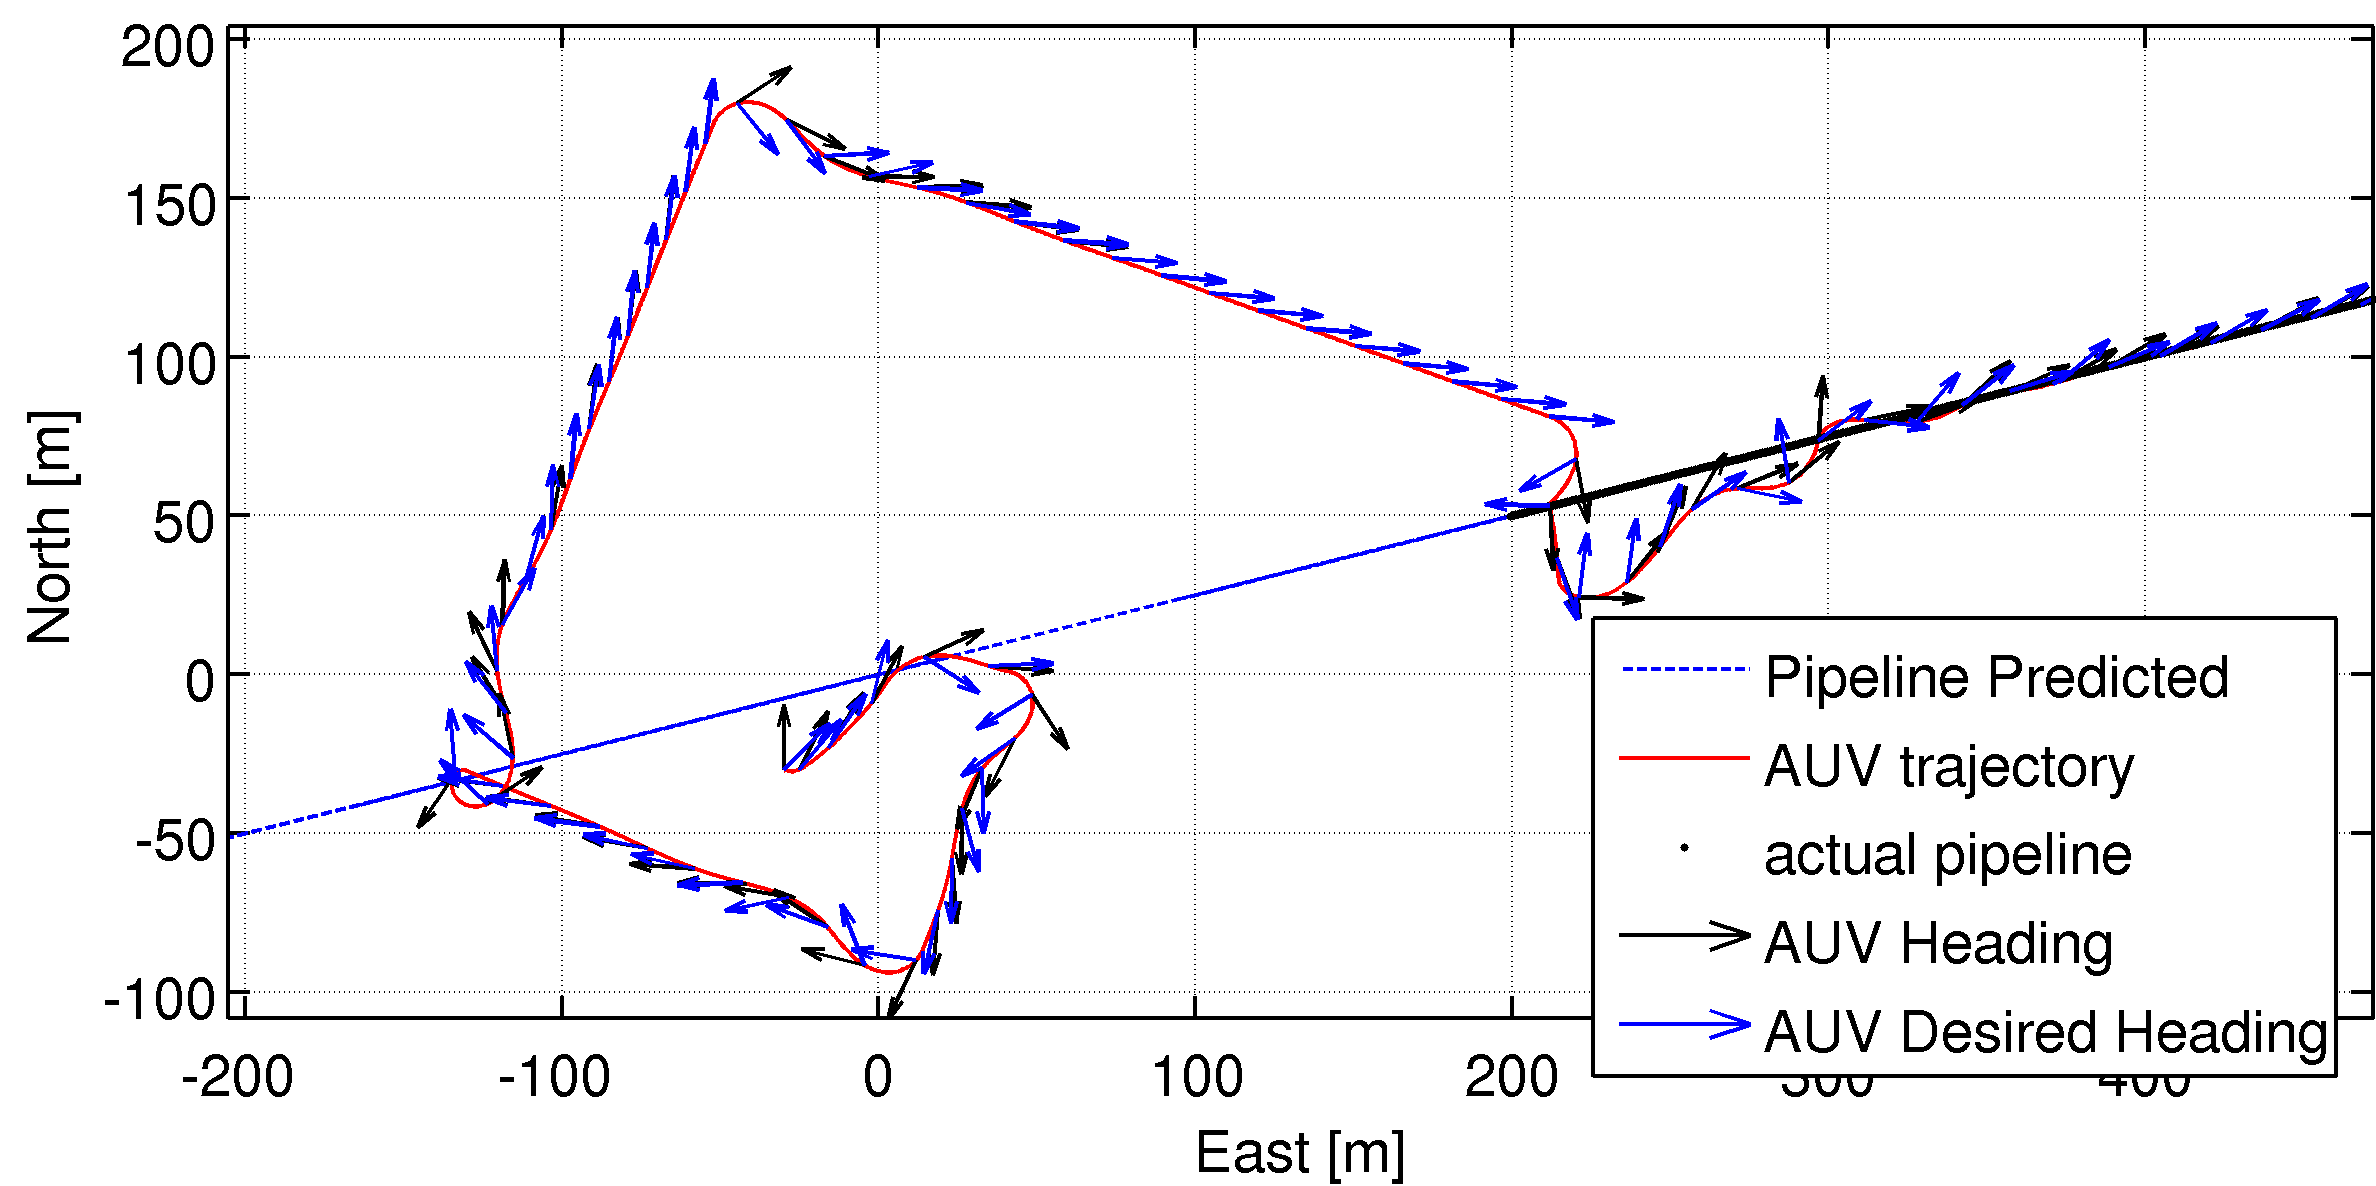
\includegraphics[width=0.8\textwidth]{pics/4th_NE_path}} 
			\caption[Trajectory plots for the 4th scenario]{Plots of the AUV Showing Trajectory, 
			Guidance Waypoints and Heading of AUV for the 4$^{\mathrm{th}}$ Scenario}
			\label{fig:ch3_4th_NE_plots}
		\end{figure}
		When the AUV reaches the initial position where the pipeline were meant to be. It does not
		make
		contact with it there, then engages in a spiral search pattern. This search pattern are
		administered by waypoints and the guidance uses the straight lines between the waypoints as
		the track to follow. This causes the more polygonal look than spiral. 
			
		From Figure~\ref{fig:ch3_4th_NE_plots} it can be seen that the AUV sometimes takes an extra
		turn
		when switching between waypoint four and five. This is due to the calculation of the desired
		heading
		angle. The \textit{matlab}-function, \textit{atan2()} are used which outputs the angle in the
		domain $(-\pi, \pi)$. Since the output from the AUV model are defined for all values, and this
		are fed back to the controller a heading reference of 0 means that it must ``unwind'' all
		turns it has done, because this accumulate the yaw value beyond $2\pi$. This is an
		implementation issue and is not caused by the theoretical guidance system. 

		The plot also shows where the filter predicts the pipeline to be. This is because the filter predicts
		the pipeline dependent on the position of the AUV. But as long as the sensors do not get a reading, the
		AUV continues on the search trajectory.

		The large overshoot when the AUV have located the pipeline are due to the current. This
		pushes the AUV away from the trajectory. The current increases the velocity in a direction and
		causes the turning in that direction to be more difficult than turning the other way. This is also a
		product of the relatively large course-changing	maneuver. This can somewhat be reduces by using
		a turn trajectory to get the AUV on the right track and the same direction as the pipeline.
		
		\begin{figure}[htbp]
			\centering
			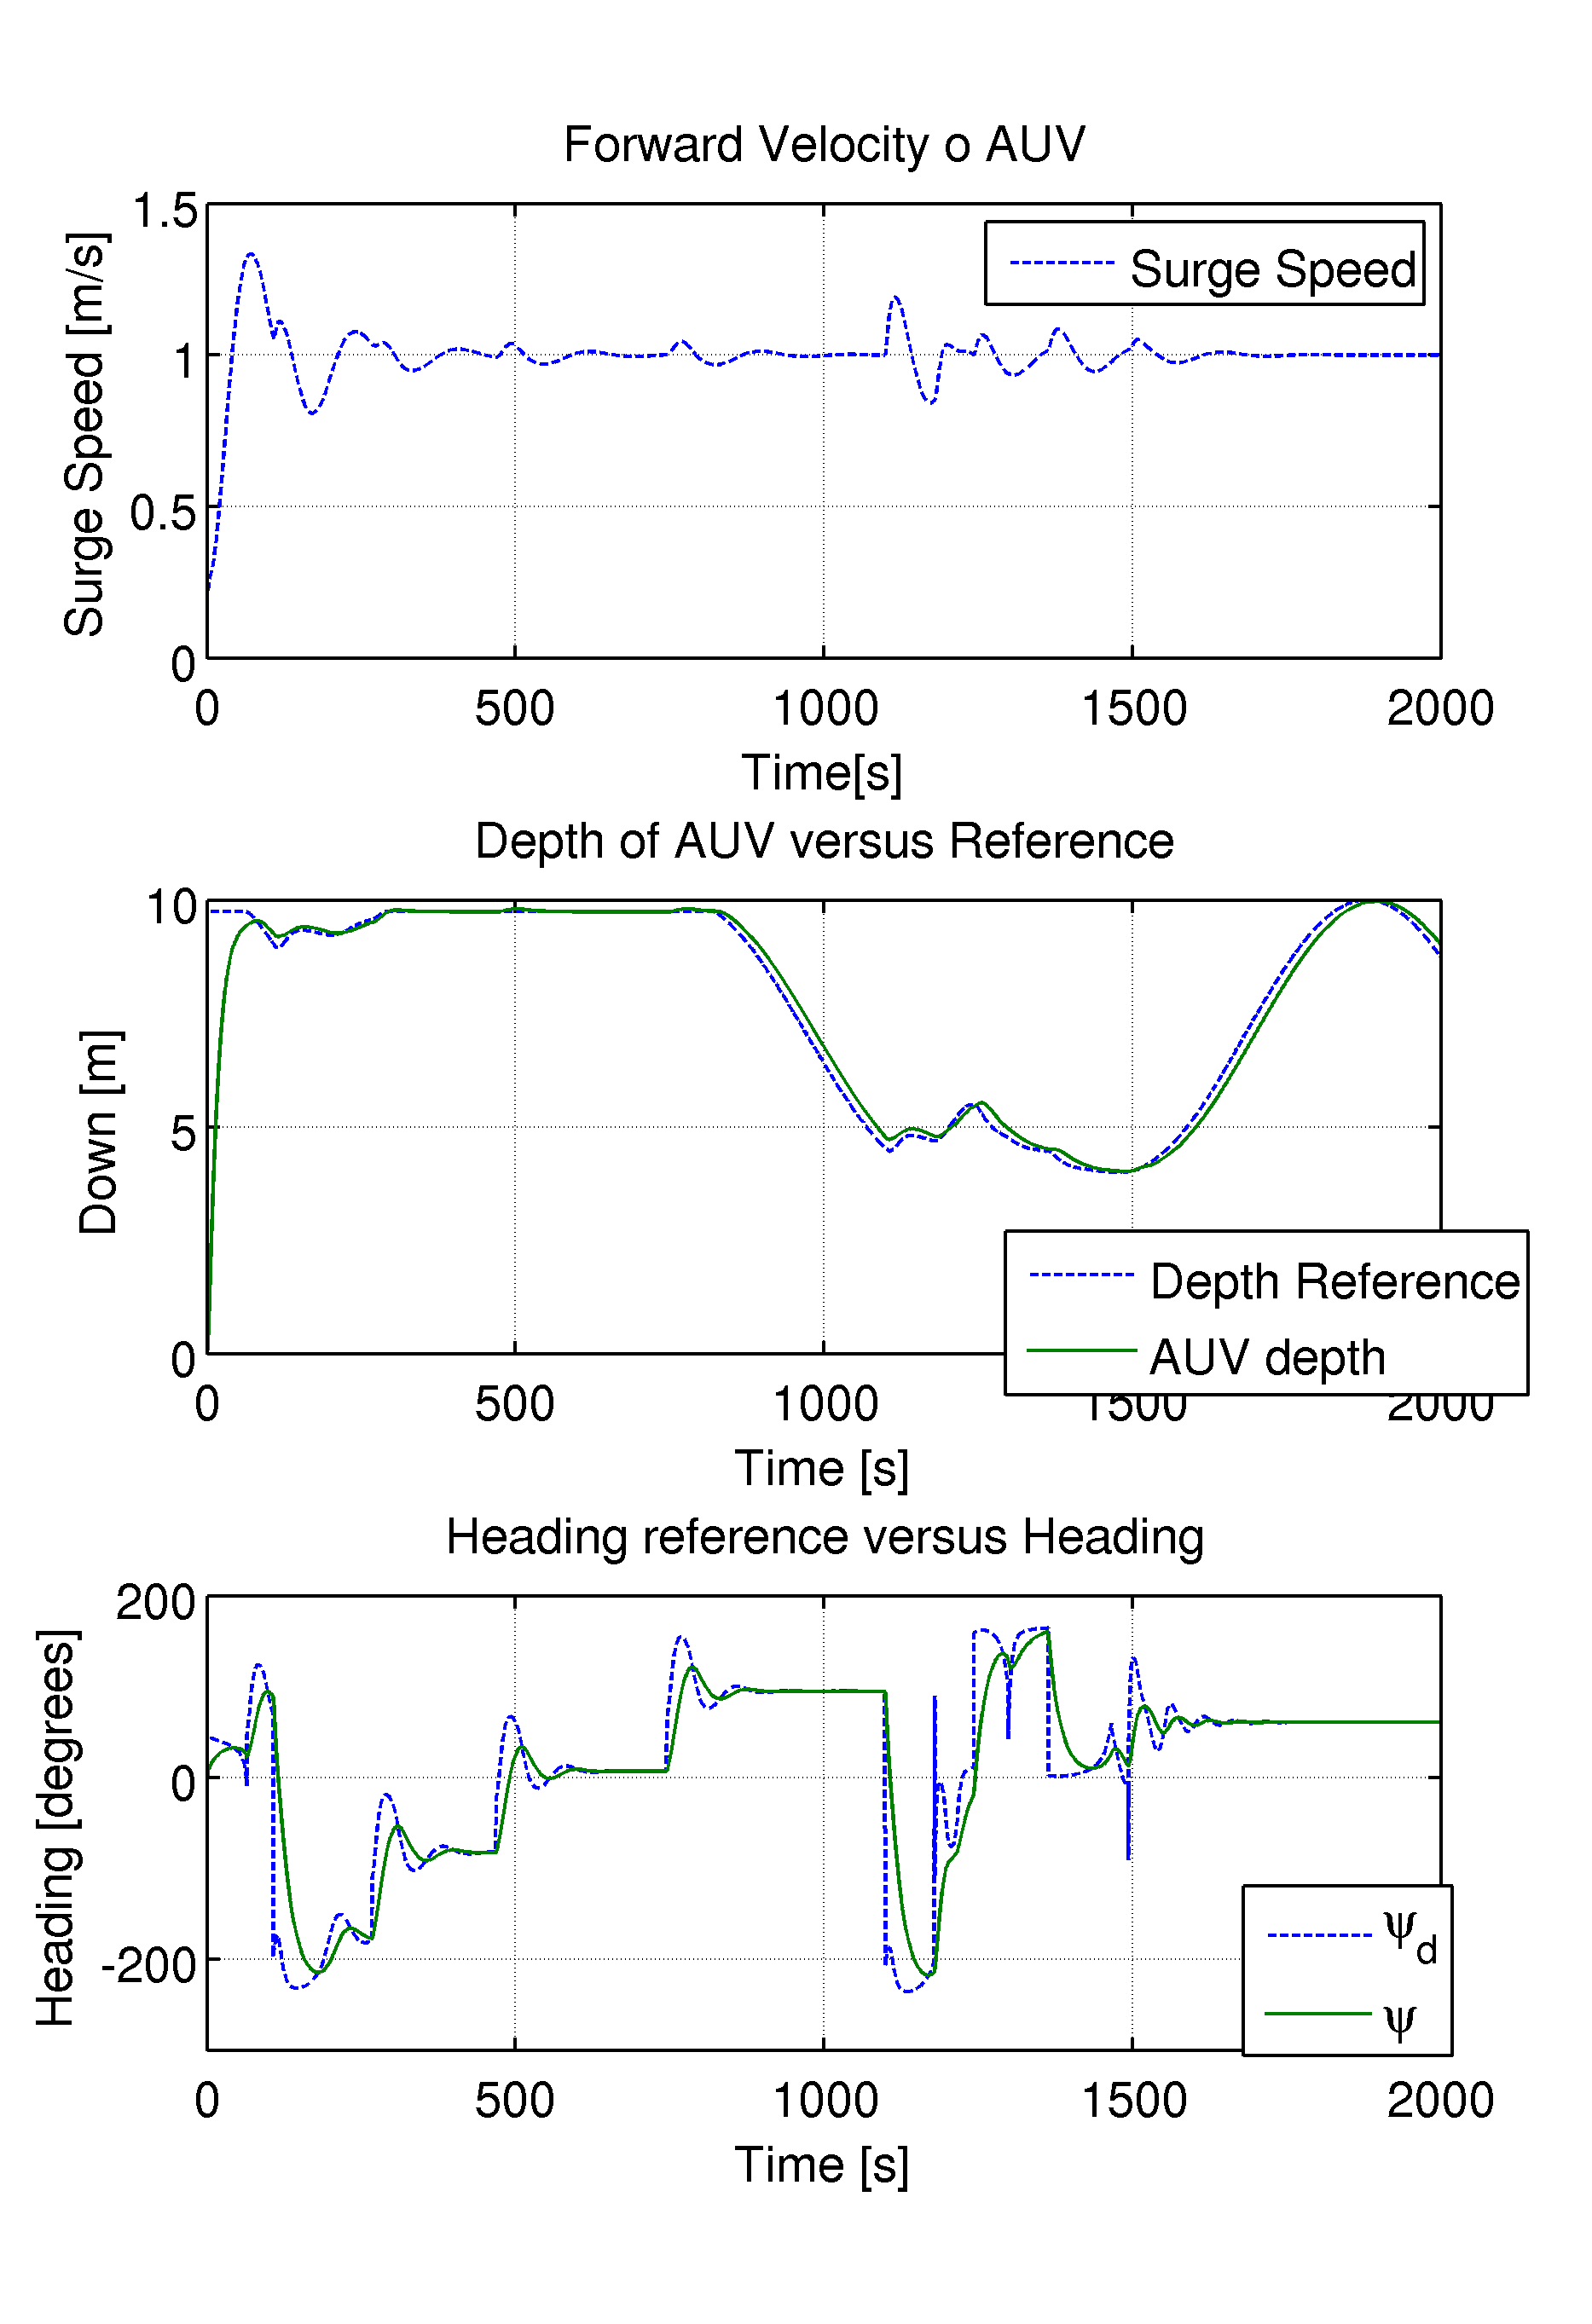
\includegraphics[width=0.70\textwidth]{pics/4th_uDpsi}
			\caption[Reference plots for the 4th scenario]{Surge-, Depth- and Heading- Reference 
			with Current influence for the fourth scenario}
			\label{fig:ch3_4th_uDpsi}
		\end{figure}
		The plots from the velocity, depth and heading references for the fourth scenario, shown in
		Figure~\ref{fig:ch3_4th_uDpsi}, are worth noting. It can be seen from the first plot in the
		figure that during large course-changing manoeuvres the surge velocity first gets a overshoot
		and then decreases under the set point of 1 m/s. This is probably because of the how the
		current are included in the simulations. We see that the course changes from around $90^\circ$
		to $-200^\circ$ over short time. The surge speed changes correspondingly in the same area.
		This is because when the course angle are about $45^\circ$, the velocity vector are parallel to
		the current, and at $-45^\circ$ the velocity vector are still parallel but in the opposite
		direction of the current. This causes the marked changes in the surge speed seen in
		Figure~\ref{fig:ch3_4th_uDpsi}. The speed controller cannot anticipate this, and therefore
		does not counteract it.

	\subsection{Test of the Prediction Filter}
		The filter data are recorded at the fourth simulation. Figure~\ref{fig:ch3_4th_filter} shows
		the error values in the predicted pipeline and the updated in the first two plots. The last
		one shows the values of the diagonal of the Kalman covariance matrix. 		
		\begin{figure}[htbp]
			\centering
			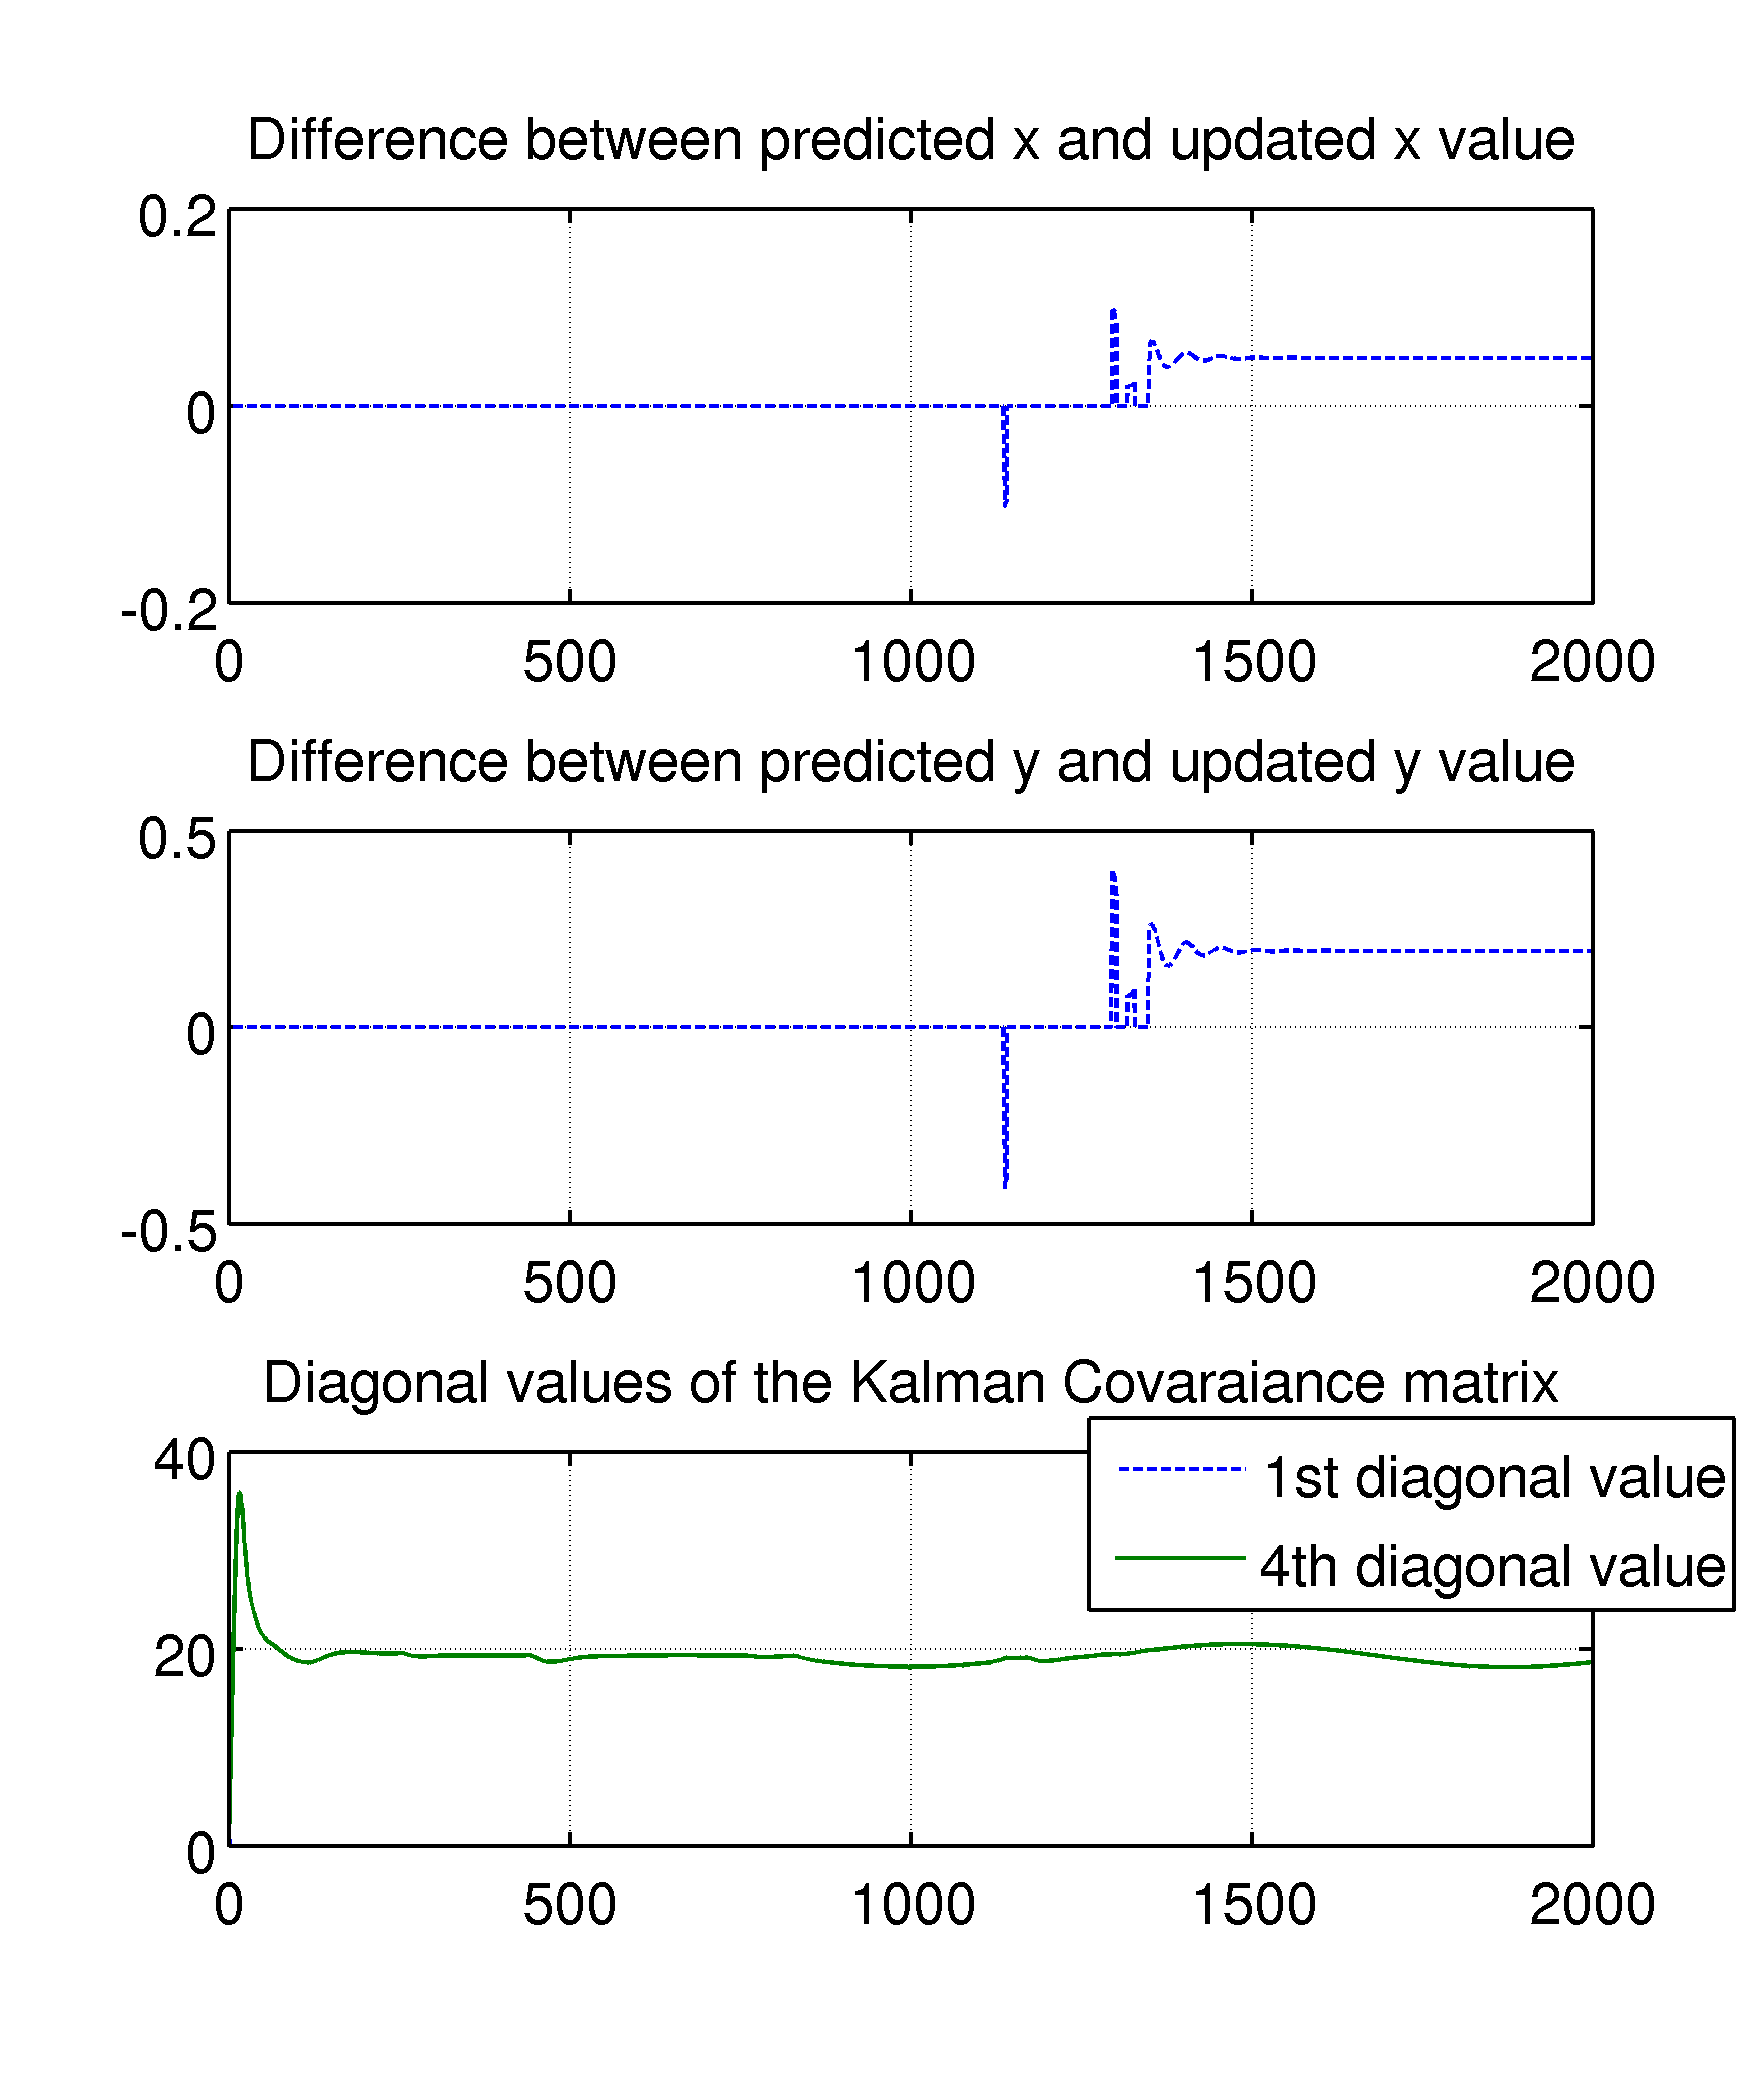
\includegraphics[width=0.70\textwidth]{pics/4th_filter}
			\caption[Filter Test]{The error values of the predicted versus updated x and y
			components of the pipeline are shown in the first two plots. The last plot shows the
			diagonal values of the covariance matrix.}
			\label{fig:ch3_4th_filter}
		\end{figure}
		
		The peaks in the error values corresponds to when the AUV makes contact with the pipeline.
		The filter updates the predicted values only when there are a valid output form the
		sensors. Also seen in the figure are constant offset when the AUV has acquired the pipeline.
		This is because the predicted values are calculated from the current position of the
		AUV, and the updated estimate from the camera gives the correct position of the pipeline. Due
		the fact that the AUV are not directly over the pipeline, this information differs and causes
		the constant error between the predicted and updated estimate. 
		Because the model used in the filter have two linear dependent states, two and two values of the
		covariance matrix are equal, i.e. the third state equals fourth and first equals second.	

		Although this filter works, it is not a very good way of doing it. The predicted position of
		the pipeline are calculated by using the position of the AUV. A better way of this is to use a
		look-up table with the predicted pipeline position. This values could be looked up when
		a measurement from the camera or other sensors were available and corrected.


